% Bantay-Baha technical specification. Build: latexmk (docs/spec/latexmkrc) or LaTeX Workshop in VS Code; see GUIDE.md.
% Results are never typed here or in sections/: they are macros from generated/numbers.tex (python scripts/make_spec.py).
\documentclass[11pt,a4paper]{article}

% ---------------------------------------------------------------- fonts and language
\usepackage[T1]{fontenc}
\usepackage[utf8]{inputenc}
\usepackage[british]{babel}
\usepackage{libertine}
\usepackage[libertine]{newtxmath}
\usepackage[varqu,scaled=0.95]{inconsolata}
\usepackage{textcomp}
\usepackage{microtype}
\usepackage{csquotes}

% ---------------------------------------------------------------- page
\usepackage[a4paper,left=25mm,right=25mm,top=24mm,bottom=26mm,headheight=14pt]{geometry}
\usepackage{xcolor}
\definecolor{ink}{HTML}{0F1E28}
\definecolor{teal}{HTML}{0A86B5}
\definecolor{amber}{HTML}{C77700}
\definecolor{alert}{HTML}{C8323F}
\definecolor{mist}{HTML}{F2F5F7}
\usepackage{fancyhdr}
\pagestyle{fancy}
\fancyhf{}
\fancyhead[L]{\small\sffamily\color{ink!70}Bantay-Baha technical specification}
\fancyhead[R]{\small\sffamily\color{ink!70}PJDSC 2026}
\fancyfoot[C]{\small\sffamily\thepage}
\renewcommand{\headrulewidth}{0.4pt}
\usepackage{titlesec}
\titleformat{\section}{\Large\sffamily\bfseries\color{ink}}{\thesection}{0.8em}{}
\titleformat{\subsection}{\large\sffamily\bfseries\color{teal}}{\thesubsection}{0.8em}{}
\titleformat{\subsubsection}{\normalsize\sffamily\bfseries\color{ink}}{\thesubsubsection}{0.8em}{}
\titlespacing*{\section}{0pt}{2.2ex plus 1ex}{1.2ex}
\titlespacing*{\subsection}{0pt}{1.8ex plus 0.8ex}{0.8ex}

% Words are never split across lines (see GUIDE.md): looser spacing instead of hyphens.
\hyphenpenalty=10000
\exhyphenpenalty=10000
\tolerance=9999
\emergencystretch=3em

% ---------------------------------------------------------------- floats, tables, lists
\usepackage{graphicx}
\graphicspath{{../results/figures/}}
\usepackage{booktabs}
\usepackage{tabularx}
\usepackage{array}
\usepackage[font=small,labelfont={bf,sf},format=plain]{caption}
\usepackage[section]{placeins}
% Floats: allow more of a text page to be float, and put float-only pages at the top instead of centring them.
\renewcommand{\topfraction}{0.85}
\renewcommand{\textfraction}{0.1}
\renewcommand{\floatpagefraction}{0.75}
\makeatletter
\setlength{\@fptop}{0pt}
\setlength{\@fpsep}{12pt plus 2fil}
\setlength{\@fpbot}{0pt plus 1fil}
\makeatother
\usepackage{enumitem}
\setlist{itemsep=0.25ex,topsep=0.6ex}
\newcolumntype{L}{>{\raggedright\arraybackslash}X}
\newcolumntype{R}{>{\raggedleft\arraybackslash}X}
\renewcommand{\arraystretch}{1.12}
\setlength{\tabcolsep}{4.5pt}

% ---------------------------------------------------------------- references
\usepackage[style=apa,backend=biber]{biblatex}
\addbibresource{refs.bib}
\usepackage{xurl}
\usepackage[hidelinks]{hyperref}
\hypersetup{colorlinks=true,linkcolor=teal,citecolor=teal,urlcolor=teal,pdftitle={Bantay-Baha technical specification},pdfsubject={PJDSC 2026}}

% ---------------------------------------------------------------- notation used in the prose
\newcommand{\code}[1]{\texttt{#1}}
% \tablerows{name} reads the generated rows generated/tab_name.tex inside a tabular. It uses TeX's primitive \input,
% because LaTeX's \input before \bottomrule fails with "Misplaced \noalign".
\makeatletter
\newcommand{\tablerows}[1]{\@@input generated/tab_#1.tex }
\makeatother
\newcommand{\stOk}{\textcolor{teal}{\textbf{done}}}
\newcommand{\stPart}{\textcolor{amber}{\textbf{partly}}}
\newcommand{\stNo}{\textcolor{alert}{\textbf{not done}}}
\usepackage{tcolorbox}
\newtcolorbox{note}{colback=amber!7,colframe=amber,boxrule=0pt,leftrule=2.5pt,arc=0pt,left=3mm,right=3mm,top=1.5mm,bottom=1.5mm,fontupper=\small}

% Figures that are typed, not computed: the proposal's assumption and figures quoted from the literature.
% (The proposal's coverage band \targetCov comes from scripts/make_spec.py COV_TARGET, which also tests against it.)
\newcommand{\proposalProvinces}{81}
\newcommand{\litNCRShare}{about 22\%}
\newcommand{\litLeptoPeak}{about two weeks}

% Results: every number below comes from the build outputs.
% Generated by scripts/make_spec.py from data/processed/ -- do not edit by hand; re-run the script.
% Every result quoted in docs/spec/sections/*.tex is one of these macros.

\newcommand{\nFiles}{501} % data/raw/MANIFEST.csv rows
\newcommand{\nSources}{22} % MANIFEST.csv sources
\newcommand{\dataGB}{7.0} % MANIFEST.csv bytes / 1e9
\newcommand{\nUnits}{85} % panel.parquet units
\newcommand{\nWeeks}{262} % panel.parquet weeks
\newcommand{\unitWeeks}{22{,}270} % panel.parquet rows
\newcommand{\dgUnits}{126} % raw DOH dengue CSV: loc.nunique()
\newcommand{\cfrSixteen}{3.9\%} % raw DOH dengue CSV: 2016 deaths / cases
\newcommand{\casesTwentyNineteen}{442k} % raw DOH dengue CSV
\newcommand{\casesTwentyTwenty}{91k} % raw DOH dengue CSV
\newcommand{\popM}{108.67~M} % panel.parquet pop
\newcommand{\rainR}{0.87} % panel: corr(chirps_7d, imerg_7d)
\newcommand{\hazUnits}{74} % panel: units with a NOAH 25-yr map
\newcommand{\hazMedian}{20\%} % panel: median hazard_any_25yr
\newcommand{\nHazNoMap}{11} % panel: units without a NOAH 25-yr map
\newcommand{\hazNoMapList}{Basilan, Batanes, Biliran, Camiguin, Davao Occidental, Guimaras, Northern Samar, Romblon, Siquijor, Sulu and Tawi-Tawi} % panel
\newcommand{\rThirtyFourMissingRolly}{29\%} % IBTrACS: Rolly gale fixes without USA R34
\newcommand{\galeFallbackKm}{150} % scenarios.run_all fixed_km
\newcommand{\nHosp}{2{,}199} % hospitals.parquet
\newcommand{\nFerry}{108} % ferries.parquet
\newcommand{\nAdmThree}{1{,}641} % scenarios_adm3.parquet municipalities
\newcommand{\susN}{0} % data/processed/sus/sus_responses.csv
\newcommand{\brierRaw}{0.089} % surge_calibration.json all_rows
\newcommand{\brierCal}{0.082} % surge_calibration.json all_rows
\newcommand{\brierClim}{0.216} % surge_calibration.json all_rows
\newcommand{\baseRatePct}{32\%} % surge_calibration.json all_rows base_rate
\newcommand{\nUncalOrigins}{13} % surge_calibration.json
\newcommand{\nUncalRows}{1{,}105} % surge_calibration.json
\newcommand{\firstCalOrigin}{8 April 2018} % surge_calibration.json
\newcommand{\gapBinLo}{0.1} % middle reliability bins, lower edge (GAP_BINS)
\newcommand{\gapBinHi}{0.7} % middle reliability bins, upper edge (GAP_BINS)
\newcommand{\gapRaw}{21\%} % surge_reliability.csv, middle bins
\newcommand{\gapCal}{7\%} % surge_reliability.csv, middle bins
\newcommand{\surgeExpected}{10\%} % 1 - forecast.SURGE_PCTL: the surge rate of a quiet year
\newcommand{\ompongRRaw}{0.22} % scenarios.parquet Ompong mean R_raw
\newcommand{\ompongR}{0.29} % scenarios.parquet Ompong mean R
\newcommand{\nDistinctR}{18} % scenarios.parquet Ompong distinct R
\newcommand{\nTies}{4} % scenarios.parquet Ompong units sharing the top R
\newcommand{\tieValue}{0.99} % scenarios.parquet Ompong top R
\newcommand{\tauMax}{3} % leadlag.pcmci_graph tau_max
\newcommand{\pcAlpha}{0.01} % leadlag.pcmci_graph pc_alpha
\newcommand{\fdrQ}{0.05} % leadlag.pcmci_graph alpha (BH q)
\newcommand{\nQuantiles}{23} % config.QUANTILES
\newcommand{\horizons}{1--4} % forecast.HORIZONS
\newcommand{\surgePctl}{90th} % forecast.SURGE_PCTL
\newcommand{\refitWeeks}{13} % forecast.rolling_origin refit_weeks
\newcommand{\nRefits}{8} % forecast.refit_dates()
\newcommand{\calMinRows}{850} % forecast.CAL_MIN_ROWS
\newcommand{\cutRatio}{2} % access.cut_off ratio
\newcommand{\cutExtraH}{1} % access.cut_off extra_h
\newcommand{\sOneAfterDays}{10} % config.S1_AFTER_DAYS
\newcommand{\nTracks}{15} % scenarios.SHIFTS
\newcommand{\nShifted}{14} % scenarios.SHIFTS without (0, 0)
\newcommand{\shiftLat}{0.5 and 1} % scenarios.SHIFTS latitude steps (degrees)
\newcommand{\shiftLon}{1} % scenarios.SHIFTS longitude steps (degrees)
\newcommand{\tierPreR}{0.3} % scenarios.TIERS preposition_R
\newcommand{\tierDeployR}{0.5} % scenarios.TIERS deploy R
\newcommand{\tierDeployA}{10\%} % scenarios.TIERS deploy A
\newcommand{\minHistory}{52} % scenarios.CATALOG_MIN_HISTORY_WEEKS
\newcommand{\leptoRainPer}{50} % lepto.RAIN_PER (mm/week per IRR unit)
\newcommand{\leptoMaxLag}{6} % lepto.LAGS
\newcommand{\leptoHeavyPctl}{90th} % lepto.HEAVY_Q
\newcommand{\nScored}{34{,}050} % eval_summary.csv n (all)
\newcommand{\relWIS}{0.544} % eval_summary.csv relWIS xgb/naive (all)
\newcommand{\covNinety}{0.85} % eval_summary.csv cov90 xgb (all)
\newcommand{\covFifty}{0.43} % eval_summary.csv cov50 xgb (all)
\newcommand{\relWISDiffPct}{46\%} % |1 - relWIS|: WIS difference to seasonal naive
\newcommand{\relWISHOne}{0.42} % eval_summary.csv relWIS xgb/naive, horizon 1
\newcommand{\relWISHTwo}{0.51} % eval_summary.csv relWIS xgb/naive, horizon 2
\newcommand{\relWISHThree}{0.59} % eval_summary.csv relWIS xgb/naive, horizon 3
\newcommand{\relWISHFour}{0.66} % eval_summary.csv relWIS xgb/naive, horizon 4
\newcommand{\covNinetyRange}{0.82--0.89} % eval_summary.csv cov90 by horizon
\newcommand{\covFiftyRange}{0.40--0.47} % eval_summary.csv cov50 by horizon
\newcommand{\covNinetyHFour}{0.82} % eval_summary.csv cov90 xgb, horizon 4
\newcommand{\relWISGraph}{0.999} % eval_summary.csv relWIS xgb/nograph
\newcommand{\relWISEnv}{1.003} % eval_summary.csv relWIS xgb/noenv
\newcommand{\relWISNoEnv}{0.542} % eval_summary.csv relWIS noenv/naive
\newcommand{\edgesEighteen}{0} % eval_graphs.csv 2018 windows
\newcommand{\edgesNineteen}{2--6} % eval_graphs.csv 2019 windows
\newcommand{\nCommon}{34{,}050} % eval_models.csv n
\newcommand{\ensRelWIS}{0.444} % eval_models.csv ens_median
\newcommand{\ensCovNinety}{90\%} % eval_models.csv ens_median cov90
\newcommand{\benchRelWISRange}{0.494--0.504} % eval_models.csv benchmarks
\newcommand{\mwXGB}{6.23} % median WIS, eval_quantiles.parquet re-scored
\newcommand{\mwEns}{6.29} % median WIS
\newcommand{\mwBenchRange}{6.54--6.83} % median WIS of the benchmarks
\newcommand{\splitThr}{198} % 90th percentile of weekly cases on the scored rows
\newcommand{\splitLoRange}{1.02--1.08} % benchmark / XGBoost mean WIS below the split
\newcommand{\splitHiRange}{0.80--0.81} % benchmark / XGBoost mean WIS above the split
\newcommand{\ensSplitLo}{0.94} % ensemble / XGBoost below the split
\newcommand{\ensSplitHi}{0.71} % ensemble / XGBoost above the split
\newcommand{\chronosLogRelWIS}{112} % bench_summary.csv chronos2_log1p
\newcommand{\chronosNoCovRelWIS}{0.480} % bench_summary.csv chronos2_nocov
\newcommand{\tabpfnLagCovRelWIS}{0.555} % bench_summary.csv tabpfn_ts_lagcov
\newcommand{\mpnnNoneRelWIS}{0.492} % bench_summary.csv mpnn_lstm_none
\newcommand{\mpnnBorderEdges}{133} % bench_mpnn_lstm.json adjacency
\newcommand{\mpnnFerryEdges}{36} % bench_mpnn_lstm.json adjacency
\newcommand{\llEdges}{8} % leadlag_meta.json pcmciplus n_edges
\newcommand{\llN}{84} % leadlag_meta.json n_series
\newcommand{\llT}{156} % leadlag_meta.json T
\newcommand{\xcEdges}{4{,}265} % leadlag_edges_xcorr.parquet
\newcommand{\sOneFloodThr}{1\%} % flooded-share threshold of make_results.stats (s1_tab, s1_muni)
\newcommand{\emsKm}{108} % EMSR312 vs Sentinel-1, km2 in the EMS AOIs
\newcommand{\sOneKm}{46} % EMSR312 vs Sentinel-1
\newcommand{\bothKm}{26} % EMSR312 vs Sentinel-1
\newcommand{\emsPrecision}{55\%} % share of S1 flood confirmed by EMS
\newcommand{\emsRecall}{24\%} % share of EMS flood S1 recovers
\newcommand{\cellsPopM}{109.4~M} % scenarios_adm3.parquet pop
\newcommand{\routeShare}{97.3\%} % scenarios_adm3.parquet
\newcommand{\meanHours}{0.24} % scenarios_adm3.parquet
\newcommand{\rasterReach}{99.5\%} % access_methods.csv baseline
\newcommand{\networkReach}{97.3\%} % access_methods.csv baseline
\newcommand{\rasterHours}{0.19} % access_methods.csv baseline
\newcommand{\networkHours}{0.24} % access_methods.csv baseline
\newcommand{\medianRatioBase}{0.62} % access_methods.csv baseline
\newcommand{\spearmanCells}{0.89} % access_methods.csv baseline
\newcommand{\cellsBoth}{321{,}701} % access_methods.csv baseline
\newcommand{\spearmanUnits}{0.95} % access_methods.csv baseline
\newcommand{\cutNetRange}{0.3--1.0~M} % scenarios.parquet observed tracks
\newcommand{\cutRasterRange}{0.6--1.6~M} % scenarios.parquet observed tracks
\newcommand{\ferriesRange}{42--100} % scenarios.parquet ferries_cancelled
\newcommand{\nProxy}{56} % shifted backtest tracks
\newcommand{\proxyCutRange}{2.3--11.3~M} % shifted tracks, network
\newcommand{\proxyRatio}{0.66} % shifted tracks: median raster / network
\newcommand{\rhoProxyRange}{0.91--0.99} % access_methods.csv shifted tracks spearman_A_units
\newcommand{\rhoObsRange}{0.78--0.86} % access_methods.csv observed tracks
\newcommand{\topTenSharedRange}{6--7} % top-10 by P shared by the methods
\newcommand{\tauMin}{0.99} % sensitivity.csv kendall_tau min
\newcommand{\tauMinRaster}{0.999} % sensitivity.csv kendall_tau_raster min
\newcommand{\tauMinAll}{0.99} % sensitivity.csv, both methods
\newcommand{\uFiveShare}{11.1\%} % Meta HRSL under-5 / cell population
\newcommand{\oSixtyShare}{6.7\%} % Meta HRSL 60+ / cell population
\newcommand{\censusUFive}{10.2\%} % 2020 census age table
\newcommand{\censusSixty}{8.5\%} % 2020 census age table
\newcommand{\uFiveCutRange}{7.9--9.5\%} % under-5 share of those cut off
\newcommand{\oSixtyCutRange}{5.2--6.2\%} % 60+ share of those cut off
\newcommand{\benchNCR}{29.7\%} % benchmark_ncr.csv share_cut
\newcommand{\nSensVariants}{9} % sensitivity.csv variants
\newcommand{\nScen}{60} % scenarios.parquet storm x track
\newcommand{\nScenTotal}{98} % backtest scenarios + catalogue storms
\newcommand{\landfallOmpong}{15 September 2018} % config.STORMS
\newcommand{\topOmpong}{Pampanga} % scenarios.parquet Ompong: highest P
\newcommand{\deployOmpong}{0} % scenarios.parquet Ompong: tier 3
\newcommand{\preposOmpong}{22} % scenarios.parquet Ompong: tier 2
\newcommand{\topTisoy}{Camarines Norte} % scenarios.parquet Tisoy: highest P
\newcommand{\deployTisoy}{0} % scenarios.parquet Tisoy: tier 3
\newcommand{\preposTisoy}{12} % scenarios.parquet Tisoy: tier 2
\newcommand{\topRolly}{Oriental Mindoro} % scenarios.parquet Rolly: highest P
\newcommand{\deployRolly}{0} % scenarios.parquet Rolly: tier 3
\newcommand{\preposRolly}{0} % scenarios.parquet Rolly: tier 2
\newcommand{\topUlysses}{Cagayan} % scenarios.parquet Ulysses: highest P
\newcommand{\deployUlysses}{0} % scenarios.parquet Ulysses: tier 3
\newcommand{\preposUlysses}{2} % scenarios.parquet Ulysses: tier 2
\newcommand{\nStormsDeploy}{0} % observed tracks with any province at deploy
\newcommand{\proxyDeployOmpong}{6--7} % Ompong shifted tracks, tier 3
\newcommand{\nCat}{38} % scenarios_catalog.parquet storms
\newcommand{\nCalCat}{24} % catalogue storms with calibrated R
\newcommand{\nAllStorms}{42} % catalogue + backtests
\newcommand{\catYearMin}{2017} % first scored storm
\newcommand{\catYearMax}{2020} % last scored storm
\newcommand{\nSkipped}{9} % catalog_storms.csv skipped for short history
\newcommand{\nLandStorms}{51} % catalog_storms.csv swath_hits_land
\newcommand{\largestCutStorms}{Kalmaegi 2019, Yutu 2018 and Vongfong 2020} % catalogue: 3 largest cut-offs
\newcommand{\highRStorms}{Bailu 2019, Podul 2019 and Kajiki 2019} % catalogue: 3 highest mean R
\newcommand{\catRhoMedian}{0.96} % access_methods_catalog.csv spearman_A_units median
\newcommand{\catRhoMin}{0.82} % access_methods_catalog.csv spearman_A_units min
\newcommand{\catRhoN}{27} % catalogue storms with any cut-off
\newcommand{\leptoNCities}{12} % lepto_events.csv cities
\newcommand{\cityObs}{3{,}036} % lepto_city_lag.csv n_obs
\newcommand{\cityCases}{1{,}685} % lepto_city_lag.csv n_cases
\newcommand{\citySigRange}{2--5} % lags whose 95% CI excludes 1
\newcommand{\cityPeakLag}{4} % joint model, highest IRR
\newcommand{\cityPeakIRR}{1.40} % joint model, highest IRR
\newcommand{\cityPeakCI}{1.40 (1.29--1.52)} % joint model, peak with CI
\newcommand{\cityCumCI}{2.45 (2.05--2.92)} % joint model, lags 0-6 cumulative
\newcommand{\heavyPeakLag}{4} % heavy-rain model peak
\newcommand{\heavyPeakCI}{2.00 (1.61--2.48)} % heavy-rain model peak
\newcommand{\natObs}{80} % lepto_national_lag.csv n_obs
\newcommand{\natPeakLag}{5} % national joint model peak
\newcommand{\natPeakCI}{1.68 (1.28--2.22)} % national joint model peak
\newcommand{\natCumCI}{4.12 (2.41--7.03)} % national cumulative
\newcommand{\natNineteenCumCI}{1.51 (0.76--3.00)} % national, 2019 only, cumulative
\newcommand{\didRUPost}{4.31 (1.72--10.85)} % lepto_events_did.csv rolly+ulysses inside x weeks 1-4
\newcommand{\didRUPre}{1.20 (0.32--4.53)} % lepto_events_did.csv rolly+ulysses placebo
\newcommand{\didOTPost}{0.81 (0.55--1.20)} % lepto_events_did.csv ompong+tisoy inside x weeks 1-4
\newcommand{\didOTPre}{2.36 (1.55--3.61)} % lepto_events_did.csv ompong+tisoy placebo
\newcommand{\sOnePairs}{48} % lepto_events.csv city-storm pairs
\newcommand{\sOnePairsSeen}{31} % pairs with radar over > 20% of the city
\newcommand{\sOnePairsFlooded}{8} % pairs with any new flood
\newcommand{\sOnePairsMax}{2.2\%} % largest flooded share
\newcommand{\statusPanel}{\stOk} % Sentinel-1 in the panel
\newcommand{\statusBench}{\stOk} % benchmarks present
\newcommand{\statusAccess}{\stOk} % raster method present
\newcommand{\statusSUS}{\stNo} % SUS responses
\newcommand{\statusLepto}{\stPart} % leptospirosis outputs
\newcommand{\rhoROmpong}{0.68} % validation.csv Ompong
\newcommand{\rhoRTisoy}{0.73} % validation.csv Tisoy
\newcommand{\rhoRRolly}{0.41} % validation.csv Rolly
\newcommand{\rhoRUlysses}{0.34} % validation.csv Ulysses
\newcommand{\rhoRRange}{0.34--0.73} % validation.csv
\newcommand{\rhoPRange}{$-$0.03--0.21} % validation.csv
\newcommand{\topTenSurgedOmpong}{7} % validation.csv top10_surge_rate x 10
\newcommand{\surgeRateOmpong}{40\%} % validation.csv surge_rate
\newcommand{\targetCov}{80--95\%} % COV_TARGET: the proposal's coverage band
\newcommand{\covNinetyConformal}{0.87} % eval_summary.csv cov90 conformal (all)
\newcommand{\nBench}{3} % benchmarks in eval_models.csv
\newcommand{\nBenchBeatXGB}{3} % benchmarks with mean WIS below XGBoost
\newcommand{\bestMeanLabel}{median ensemble} % eval_models.csv: lowest relWIS_vs_naive
\newcommand{\bestMeanRelWIS}{0.444} % eval_models.csv
\newcommand{\bestMeanCov}{90\%} % eval_models.csv
\newcommand{\bestMedianLabel}{XGBoost + graph (ours)} % lowest median WIS
\newcommand{\bestMedianWIS}{6.23} % lowest median WIS
\newcommand{\surgeRateTisoy}{5\%} % validation.csv surge_rate
\newcommand{\topTenSurgedTisoy}{0} % validation.csv top10_surge_rate x 10
\newcommand{\statusRelWIS}{\stOk} % relWIS < 1
\newcommand{\statusCov}{\stOk} % cov90 inside COV_TARGET at every horizon

% Conditions behind qualitative claims: \if<Name> ... \else ... \fi in the prose.
\newif\ifForecastBeats\ForecastBeatstrue % relWIS xgb/naive < 1 (all horizons pooled)
\newif\ifRelBelowAllH\RelBelowAllHtrue % relWIS < 1 at every horizon
\newif\ifCovInsideAllH\CovInsideAllHtrue % cov90 inside COV_TARGET at every horizon
\newif\ifCovFourNearFloor\CovFourNearFloortrue % 4-week cov90 within 0.03 of the floor
\newif\ifCovFiftyNarrow\CovFiftyNarrowtrue % every 50% interval covers less than 50%
\newif\ifCovFiftyWide\CovFiftyWidefalse % every 50% interval covers more than 50%
\newif\ifConformalSimilar\ConformalSimilartrue % conformal and model 90% coverage within 0.03
\newif\ifGraphHelps\GraphHelpsfalse % relWIS xgb/nograph < 0.98
\newif\ifEnvHelps\EnvHelpsfalse % relWIS xgb/noenv < 0.98
\newif\ifAnyBenchBeatsXGB\AnyBenchBeatsXGBtrue % some benchmark below XGBoost on mean WIS
\newif\ifMeanMedianDiffer\MeanMedianDiffertrue % the best model on mean WIS is not the best on median WIS
\newif\ifBenchWinHigh\BenchWinHightrue % benchmarks beat XGBoost above the 90th percentile of cases and lose below it
\newif\ifEnsGainsBoth\EnsGainsBothtrue % ensemble below XGBoost in both halves
\newif\ifChronosLogCollapsed\ChronosLogCollapsedtrue % chronos2_log1p relative WIS above 2
\newif\ifChronosCovHelps\ChronosCovHelpsfalse % chronos2 with covariates below without
\newif\ifMpnnGraphSame\MpnnGraphSametrue % MPNN-LSTM with / without graph within 0.01
\newif\ifCalImproves\CalImprovestrue % Brier calibrated < raw
\newif\ifRawUnderConfident\RawUnderConfidenttrue % middle bins: observed above raw R on average
\newif\ifCalGapSmaller\CalGapSmallertrue % largest middle-bin gap shrinks
\newif\ifBaseRateHigh\BaseRateHightrue % base rate well above the quiet-year rate
\newif\ifOmpongRRises\OmpongRRisestrue % Ompong mean R calibrated > raw
\newif\ifXcorrMany\XcorrManytrue % cross-correlation keeps 10x the PCMCI+ links
\newif\ifEMSRecallLow\EMSRecallLowtrue % Sentinel-1 recovers under half of the EMS area
\newif\ifRasterReachMore\RasterReachMoretrue % normal day: raster reaches more people
\newif\ifRasterFaster\RasterFastertrue % normal day: raster trips shorter
\newif\ifMethodsRankAlike\MethodsRankAliketrue % normal day: Spearman over cells >= 0.7
\newif\ifRasterMoreSOne\RasterMoreSOnetrue % observed tracks: raster cuts off more people
\newif\ifRasterMoreProxy\RasterMoreProxyfalse % proxy tracks: median raster / network > 1
\newif\ifProxyAgreesBetter\ProxyAgreesBettertrue % rho of A: every proxy track above every observed track
\newif\ifGaleNoEffect\GaleNoEffecttrue % every gale-fallback variant leaves P's ranking unchanged
\newif\ifSensStable\SensStabletrue % Kendall's tau >= 0.95 for every variant
\newif\ifHRSLUnderOld\HRSLUnderOldtrue % HRSL 60+ share below the census
\newif\ifHRSLOverYoung\HRSLOverYoungtrue % HRSL under-5 share above the census
\newif\ifRRanksWell\RRanksWelltrue % rho(R, observed) >= 0.5 for both 2018-2019 storms
\newif\ifPLessThanR\PLessThanRtrue % rho(P) < rho(R) for both 2018-2019 storms
\newif\ifCatLargestLowR\CatLargestLowRfalse % the 3 largest cut-offs all have R below the catalogue median
\newif\ifCatHighRNineteen\CatHighRNineteentrue % the 3 highest-R storms are all 2019
\newif\ifCitySig\CitySigtrue % some city lag has a 95% CI above 1
\newif\ifCityPeakLater\CityPeakLatertrue % city peak later than two weeks
\newif\ifNatNineteenNull\NatNineteenNulltrue % 2019-only national cumulative CI includes 1
\newif\ifRUPostSig\RUPostSigtrue % Rolly+Ulysses inside x weeks 1-4: CI excludes 1
\newif\ifRUPlaceboOK\RUPlaceboOKtrue % Rolly+Ulysses placebo CI includes 1
\newif\ifOTPostSig\OTPostSigfalse % Ompong+Tisoy inside x weeks 1-4: CI excludes 1
\newif\ifOTPlaceboOK\OTPlaceboOKfalse % Ompong+Tisoy placebo CI includes 1
\newif\ifLeptoFloodFew\LeptoFloodFewtrue % fewer than 10 flooded city-storm pairs
\newif\ifSUSPending\SUSPendingtrue % fewer than three SUS responses
\newif\ifNHFRMissing\NHFRMissingtrue % status.json: nhfr missing


\title{\sffamily\bfseries Bantay-Baha\\[0.4ex]\Large\mdseries Technical specification}
\author{\normalsize PJDSC 2026}
\date{\normalsize Generated from the pipeline outputs on \today}

\begin{document}

\maketitle
\thispagestyle{fancy}

% !TEX root = ../main.tex
\begin{abstract}
\noindent Bantay-Baha ranks Philippine provinces for action before a typhoon arrives. It combines the probability $R$ that a province's dengue cases surge in the next four weeks with the share $A$ of its people that the storm cuts off from a hospital, and ranks provinces by the priority $P = R \times A$. This specification describes the data, the method of every layer and how each was evaluated; every result in it is computed from the pipeline outputs at build time. Over \nScored{} rolling-origin forecasts in 2018--2019, a multi-quantile gradient-boosted model reaches a relative weighted interval score (WIS) of \relWIS{} against a seasonal-naive forecast, with a 90\% interval coverage of \covNinety{}; its median ensemble with \nBench{} benchmark models reaches \ensRelWIS{}. For the four backtest typhoons, \cutNetRange{} people lose their route to a hospital on the road and ferry network when roads are cut by flood observed from radar. The lead-lag outbreak graph between provinces keeps \llEdges{} links; at one to four weeks its features \ifGraphHelps improve\else do not improve\fi{} the forecast, and the rain and flood features \ifEnvHelps do\else do not either\fi.
\end{abstract}

\tableofcontents
\clearpage

% !TEX root = ../main.tex
\section{Summary}
\label{sec:summary}

Bantay-Baha joins three graphs into one ranking: a flood-exposure layer (rain, river routing, observed and mapped flood), a lead-lag outbreak graph learned between provinces, and a road and ferry access graph that a typhoon cuts. A quantile forecast of dengue gives the probability $R$ that a province's next four weeks exceed its usual bad month; two access methods give the share $A$ of people cut off from a hospital; the priority is $P = R \times A$. Dengue forecasting in the Philippines has been studied at province level before \parencite{buczak2014}, and typhoon flooding is followed by leptospirosis \parencite{balbuena2010}; what is new here is the combination with storm-driven access loss, ranked for any typhoon track. Every number in this document was computed by the build (\code{build.bat}) from the raw files and written into it by \code{scripts/make\_spec.py}.

\subsection{Findings}

\begin{itemize}
\item \textbf{The forecast beats the bar.} Multi-quantile XGBoost reaches a relative WIS of \relWISHOne{} at one week and \relWISHFour{} at four weeks over \nScored{} rolling-origin forecasts in 2018--2019 (Section~\ref{sec:forecast}).
\item \textbf{Benchmarked, and beaten on the mean.} Two zero-shot foundation models and a graph neural network reach relative WIS \benchRelWISRange{}, all below XGBoost; their median ensemble with XGBoost is best (\ensRelWIS{}, 90\% coverage \ensCovNinety{}). On the median WIS XGBoost is best (\mwXGB{} against \mwBenchRange{}): the benchmarks win on high-count epidemic weeks. Storm scenarios still use XGBoost, the only model that takes the storm track (Section~\ref{sec:models}).
\item \textbf{Two honest null results.} Lead-lag graph features do not help (graph against no graph, relative WIS \relWISGraph{}), nor do rain, river, storm and flood features (\relWISEnv{}). At one to four weeks, recent cases and the season carry the skill.
\item \textbf{Surge probability $R$, recalibrated.} Isotonic regression on past rolling-origin forecasts only lowers the Brier score from \brierRaw{} to \brierCal{} (\brierClim{} for always predicting the base rate) and removes the model's under-confidence in the middle range (Section~\ref{sec:calibration}).
\item \textbf{The ranking points at the right places.} The Spearman correlation of $R$ with next-four-week incidence is \rhoROmpong{} for Ompong and \rhoRTisoy{} for Tisoy; \topTenSurgedOmpong{} of Ompong's ten highest-priority provinces surged against a \surgeRateOmpong{} base rate (Section~\ref{sec:validation}).
\item \textbf{Access loss, two methods.} For the observed tracks, with roads cut by Sentinel-1 observed flood, \cutNetRange{} people lose their route on the road and ferry network and \cutRasterRange{} on the friction raster; the gap is reported as a range. Gale swaths cancel \ferriesRange{} of \nFerry{} ferry routes, and Kendall's $\tau$ of the ranking under \nSensVariants{} setting changes is at least \tauMinAll{} (Section~\ref{sec:access}).
\item \textbf{Leptospirosis, the stretch goal.} In \leptoNCities{} cities, rain is followed by leptospirosis \citySigRange{} weeks later (peak incidence rate ratio \cityPeakIRR{} per +\leptoRainPer{}~mm/week at lag \cityPeakLag{}); nothing is extrapolated to provinces (Section~\ref{sec:lepto}).
\end{itemize}

\begin{note}
\textbf{Not in these results:} System Usability Scale responses from target users (\susN{} so far; the test is built into the dashboard) and the official facility registry (hospitals are the OpenStreetMap and hazard-map fallback). The scorecard against the proposal is in Section~\ref{sec:scorecard}.
\end{note}

Figure~\ref{fig:timeline} shows the forecast target over the whole period, with the four backtest typhoons.

\begin{figure}[htbp]
\centering
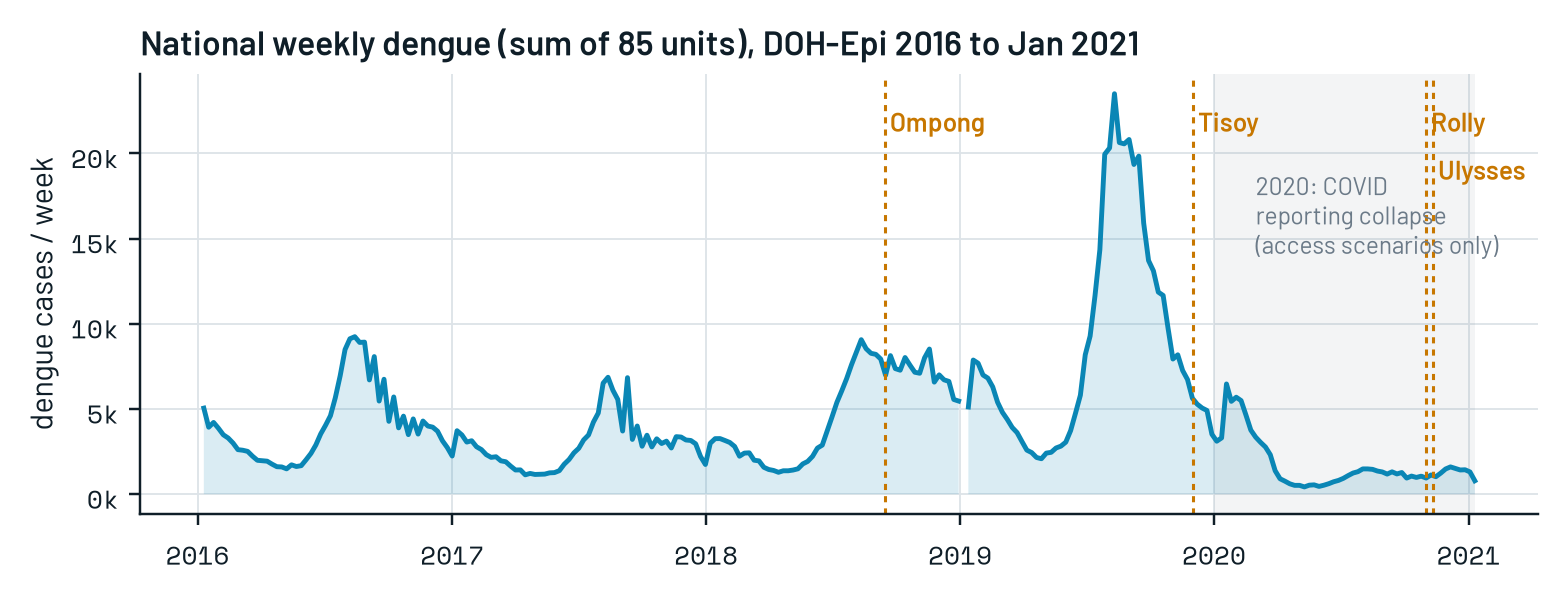
\includegraphics[width=\linewidth]{f01_timeline}
\caption{The forecast target: weekly dengue cases from the Department of Health (DOH), summed over the \nUnits{} harmonised units, with the four backtest typhoons. 2020 is used for access scenarios only.}
\label{fig:timeline}
\end{figure}

% !TEX root = ../main.tex
\section{Data}
\label{sec:data}

\subsection{Acquisition}

\nFiles{} files from \nSources{} sources (\dataGB{}~GB) are listed in \code{data/raw/MANIFEST.csv} with their size and SHA-256 hash; all were verified on disk before this build. Open sources come from \code{scripts/download\_data.py}, Google Earth Engine sources from \code{scripts/download\_gee.py} \parencite{gorelick2017}, and the team shares them through a private bucket (\code{setup.bat}, every file checked against the manifest). Table~\ref{tab:sources} lists them; the two manual sources were not needed (last rows).

The forecast target is the DOH weekly dengue series on the Humanitarian Data Exchange (HDX) \parencite{doh2021}. Population comes from the 2020 census \parencite{psa2021} and WorldPop \parencite{tatem2017}, boundaries and join keys from the common operational administrative boundaries (COD-AB) \parencite{psa2025}, storms from the International Best Track Archive for Climate Stewardship (IBTrACS) \parencite{knapp2010}, rain from CHIRPS \parencite{funk2015} and IMERG \parencite{huffman2023}, rivers from HydroRIVERS \parencite{lehner2013}, roads from OpenStreetMap (OSM) \parencite{osm2026} and observed flood for Ompong from the Copernicus Emergency Management Service (EMS) \parencite{copernicus2018}.

\begin{table}[htbp]
\centering
\caption{Data sources, as recorded in the manifest (files and size on disk).}
\label{tab:sources}
\footnotesize
\begin{tabularx}{\linewidth}{@{}>{\ttfamily}l L L l r r@{}}
\toprule
\normalfont folder & dataset & role & from & files & MB \\
\midrule
\tablerows{sources}
\bottomrule
\end{tabularx}
\end{table}

\subsection{Harmonised units}

The DOH file has \textbf{\dgUnits{} reporting units, not \proposalProvinces{} provinces}: provinces mixed with highly urbanised and component cities, plus misspellings (NUEVA VISCAYA, SISQUIJOR, BASILIG CITY for Bislig). COD-AB uses current boundaries (Maguindanao split in 2022, the Special Geographic Area created in 2024). The reviewed crosswalk in \code{data/crosswalks/} folds cities into their province and undoes the post-2020 changes, giving \textbf{\nUnits{} units}; every dengue unit resolves and every unit has data. A unit-week counts only if every member reported (missing otherwise, never zero). Deaths are not used (the 2016 case fatality of \cfrSixteen{} is far above the other years), and 2020 fell to \casesTwentyTwenty{} cases against \casesTwentyNineteen{} in 2019 under COVID-19, so 2020 is never a forecast target.

\subsection{Population}

The 2020 census table's municipal codes are the old 9-digit Philippine Standard Geographic Code (PSGC) and do not join to COD-AB for the highly urbanised cities, post-split Maguindanao and the Special Geographic Area. The table's own \emph{Province} column already places cities in their province, so units are summed on it: \popM{} people.

\subsection{Flood-exposure inputs}

Figure~\ref{fig:coverage} shows how much of the \nUnits{}~$\times$~\nWeeks{} panel (\unitWeeks{} unit-weeks) each input fills. Rain from CHIRPS and IMERG agrees (weekly $r = \rainR$). River routing accumulates CHIRPS rain down the HydroRIVERS network. The flood hazard maps of the Nationwide Operational Assessment of Hazards (NOAH) at a 25-year return period cover \hazUnits{} of \nUnits{} units; the median unit has \hazMedian{} of its people in a hazard zone. The \nHazNoMap{} units with no map are \textbf{missing, not zero}: \hazNoMapList{}.

Storm exposure uses every Western Pacific track of 2016--2020 from IBTrACS, with the gale radius from the United States 34-knot radius, else the Japan Meteorological Agency (JMA) 30-knot radius, else a fixed \galeFallbackKm{}~km. The United States radius is missing on \rThirtyFourMissingRolly{} of Rolly's gale-strength fixes (JMA fills them)\ifGaleNoEffect; the fixed fallback never applies to the four storms (Section~\ref{sec:validation})\fi.

\begin{figure}[htbp]
\centering
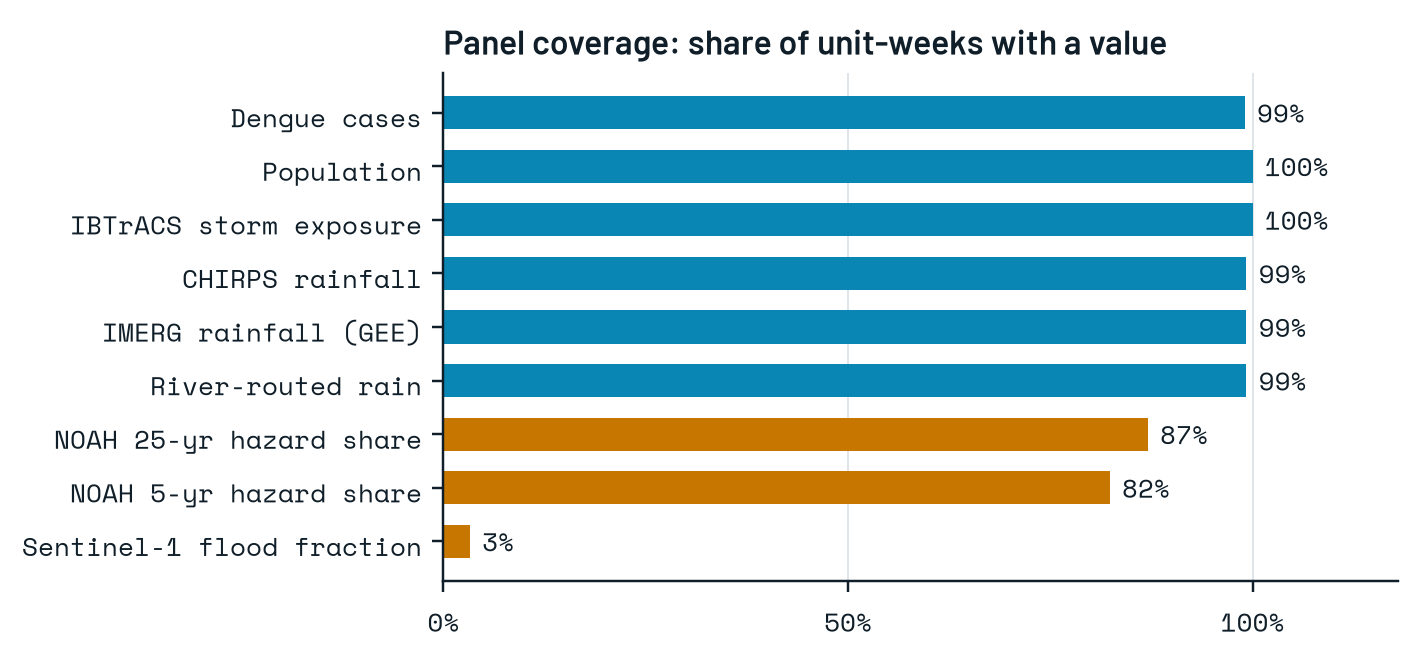
\includegraphics[width=0.72\linewidth]{f02_coverage}
\caption{Coverage of the unit-week panel: the share of unit-weeks with a value, per input. Sentinel-1 is filled only for the four landfall windows, by design.}
\label{fig:coverage}
\end{figure}

% !TEX root = ../main.tex
\section{Methods}
\label{sec:methods}

\subsection{Layer 1: flood exposure}

Each unit-week carries the CHIRPS and IMERG rain of that week and its lags, the upstream-mean rain routed down the river network and weighted by discharge, the storm exposure (whether the unit lies inside a gale swath that week), the share of people in a NOAH hazard zone (25- and 5-year return periods, missing where there is no map) and, for the four backtest storms, the new-flood share seen by Sentinel-1 (Section~\ref{sec:flood}). The Sentinel-1 feature starts in the week that contains landfall plus \sOneAfterDays{} days, the end of its after-image window, so no forecast origin sees radar from its own future.

\subsection{Layer 2: lead-lag outbreak graph}

The series is $\log(1 + \text{incidence})$, differenced over 52 weeks to remove the season and standardised inside the training window. PCMCI+, a causal discovery algorithm for time series \parencite{runge2019, runge2020}, runs with partial-correlation tests at lags 1 to \tauMax{} weeks and $\alpha_{\text{PC}} = \pcAlpha$; a lagged link between two provinces is kept when its false discovery rate (FDR) q-value is below \fdrQ{} \parencite{benjamini1995}. On pure-noise checks PCMCI+ without this step returned many false links. PageRank on the reversed graph scores sentinel provinces \parencite{page1999}, Louvain finds communities \parencite{blondel2008}, and lagged cross-correlation with the same FDR filter is the baseline graph.

\subsection{Forecast and surge probability}

One pooled XGBoost model \parencite{chen2016} per horizon (\horizons{} weeks) is trained with a multi-quantile objective at the \nQuantiles{} quantile levels of the FluSight challenge of the United States Centers for Disease Control and Prevention, on $\log(1 + \text{incidence})$, and back-transformed to cases. The features are lagged incidence, the same week of the previous year, the week of the year, rain and river lags, storm exposure, NOAH hazard, Sentinel-1 flood and leader signals from the graph; Shapley additive explanations (SHAP) give the drivers shown on the dashboard \parencite{lundberg2017}. A direct four-week model gives $R$, the probability of exceeding the unit's \surgePctl{} percentile of four-week incidence in the training window. $R$ is then recalibrated by isotonic regression \parencite{zadrozny2002}, fitted only on earlier rolling-origin forecasts whose outcome was known at the origin, and only once \calMinRows{} such outcomes exist.

\textbf{Benchmarks} are scored on exactly the same rows: Chronos-2 \parencite{ansari2025} and TabPFN-TS \parencite{hoo2025} zero-shot, each origin's forecast made from that unit's own past only; a message-passing graph network with a long short-term memory (MPNN-LSTM) \parencite{panagopoulos2021} trained on the same \refitWeeks{}-week rolling refits; and the element-wise median of the \nQuantiles{} quantiles of XGBoost and the three (the ensemble).

\subsection{Evaluation protocol}

\textbf{Rolling origin, never a random split} (Figure~\ref{fig:rolling}). From January 2018 to December 2019 the model, the graph and the surge thresholds are refit every \refitWeeks{} weeks (\nRefits{} refits) on data up to the refit date, and every origin until the next refit is forecast from them. The scores are the WIS on case counts \parencite{bracher2021}, the relative WIS against a seasonal-naive forecast (the same week of the previous year, with its empirical quantiles), the 50\% and 90\% interval coverage, and an online conformal 90\% band built from past errors only \parencite{gibbs2021}.

\begin{figure}[htbp]
\centering
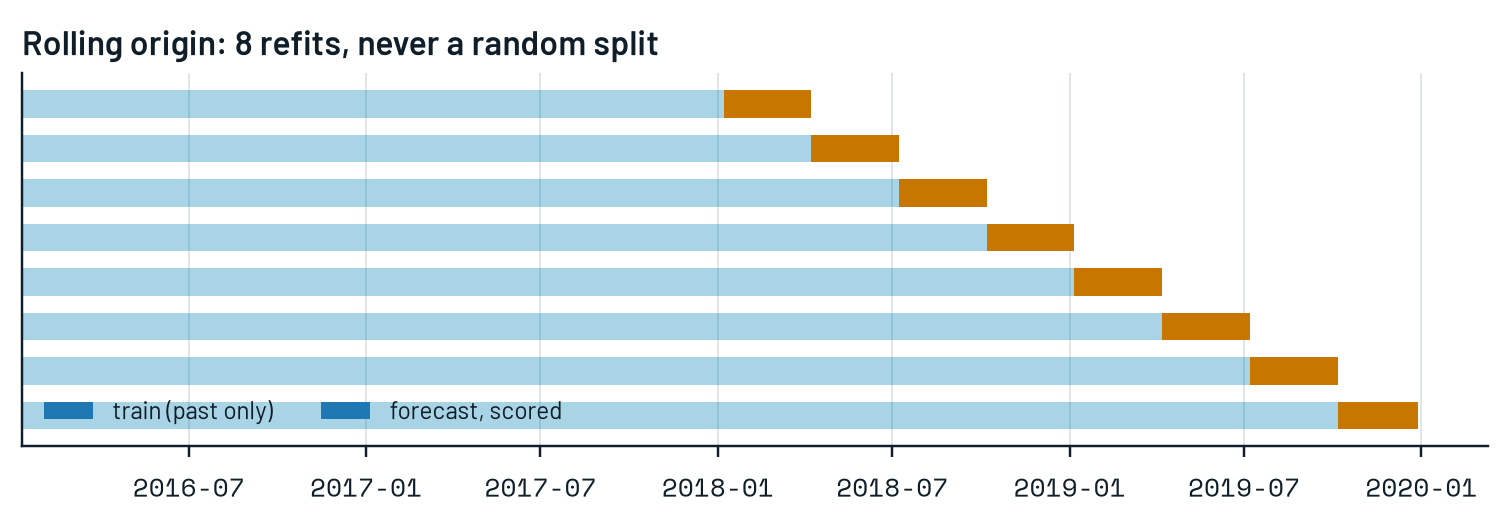
\includegraphics[width=\linewidth]{f14_rolling}
\caption{Rolling-origin evaluation: each block is forecast only from a model trained on the data before it.}
\label{fig:rolling}
\end{figure}

\subsection{Layer 3: access, two methods}

\textbf{Network.} OSM highways become a graph of junctions; roll-on/roll-off (RoRo) ferry routes are extra edges (crossing time plus half the headway); hospitals are the Humanitarian OpenStreetMap Team (HOT) health facilities plus NOAH name-matched facilities (\nHosp{}). WorldPop is summed to 1~km cells, each joined to the nearest road node, and a multi-source Dijkstra search gives the hours to the nearest hospital.

\textbf{Raster.} A cost-distance search from the same hospitals runs over the motorised friction surface of the Malaria Atlas Project (MAP) \parencite{weiss2020}, with the sea impassable except along the same ferry lines.

\textbf{Storms} apply the same rules to both methods: ferries crossing the gale swath are cancelled; roads (or cells) in observed flood (Sentinel-1, observed tracks) or in NOAH high hazard inside the swath (shifted tracks) are cut, and medium hazard slows them. A cell is cut off if it loses its route, or if its trip grows at least \cutRatio{}-fold and by more than \cutExtraH{}~h \parencite[after][]{petricola2022}. The network gives $A$, $P$ and the action tier; the per-unit minimum and maximum of the two methods give the ranges $A_{\text{lo}}$--$A_{\text{hi}}$ and $P_{\text{lo}}$--$P_{\text{hi}}$. Under-5 and 60+ people come from the High Resolution Settlement Layer (HRSL) \parencite{tiecke2017}, summed to the same cells; a cell's vulnerable people are cut off when the cell is.

% !TEX root = ../main.tex
\section{Forecast skill}
\label{sec:forecast}

Table~\ref{tab:eval} gives the rolling-origin scores of XGBoost by horizon. \textbf{The targets are met.} The relative WIS is below 1 at every horizon (\relWISHOne{} to \relWISHFour{}) and the 90\% coverage is inside the proposal's \targetCov{} band at every horizon (four weeks is close to the floor at \covNinetyHFour{}). The 50\% intervals are a little narrow (\covFiftyRange{}). The online conformal band reaches a similar coverage, a sign that the quantiles are not badly miscalibrated.

\begin{table}[htbp]
\centering
\caption{Forecast skill of XGBoost by horizon: WIS on case counts for XGBoost, XGBoost without the graph features and the seasonal-naive forecast; relative WIS against the naive forecast and against the no-graph model; empirical coverage.}
\label{tab:eval}
\footnotesize
\begin{tabular}{@{}l r r r r r r r r r@{}}
\toprule
horizon & $n$ & WIS & WIS no graph & WIS naive & rel.\ WIS & graph / no graph & cov.\ 50 & cov.\ 90 & cov.\ 90 conformal \\
\midrule
\tablerows{eval}
\bottomrule
\end{tabular}
\end{table}

\subsection{What carries the skill}

Table~\ref{tab:skill} compares the full model with its ablations, all scored on the same rows. XGBoost has a \relWISLowerPct{} lower WIS than the same week of the previous year. The graph adds nothing: it has \edgesEighteen{} links in the 2018 windows and \edgesNineteen{} in 2019, so leader signals are empty for most provinces. Rain, river, storm and flood features add nothing either. Two likely reasons, not tested: in a four-year panel rain moves with the season, so the season features already carry it, and any effect at lags beyond four weeks is outside this horizon. Figure~\ref{fig:fan} shows the forecasts for Cagayan, Ompong's landfall province.

\begin{table}[htbp]
\centering
\caption{Ablations: relative WIS of each comparison on the same rolling-origin rows.}
\label{tab:skill}
\small
\begin{tabularx}{\linewidth}{@{}l r L@{}}
\toprule
comparison & relative WIS & reading \\
\midrule
XGBoost against seasonal naive & \relWIS{} & \relWISLowerPct{} lower WIS than the same week last year \\
with against without graph leader features & \relWISGraph{} & no gain from the graph \\
with against without rain, river, storm and flood & \relWISEnv{} & \relWIS{} against \relWISNoEnv{} relative to seasonal naive \\
\bottomrule
\end{tabularx}
\end{table}

\begin{figure}[htbp]
\centering
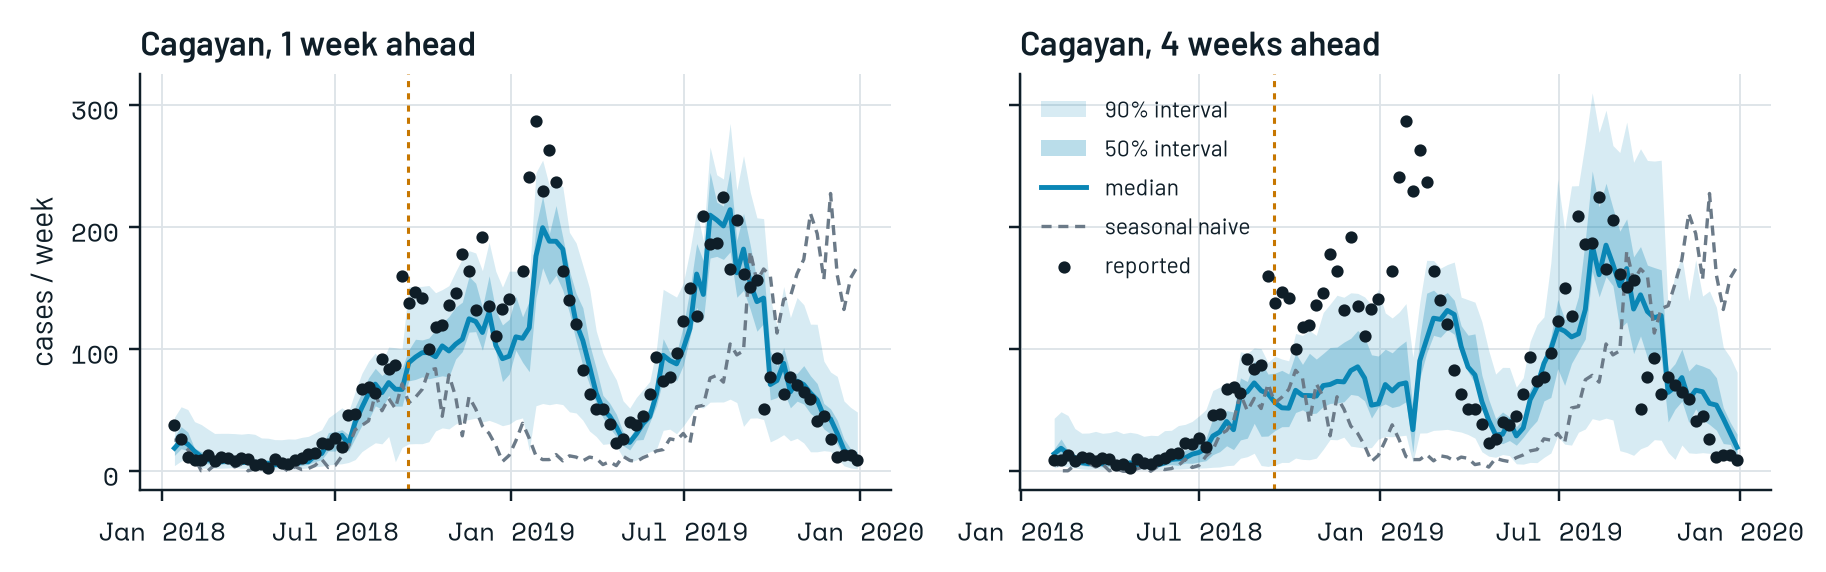
\includegraphics[width=\linewidth]{f05_fan}
\caption{Rolling-origin forecasts for Cagayan, one and four weeks ahead; the dashed line marks Ompong's landfall.}
\label{fig:fan}
\end{figure}

\subsection{Model comparison}
\label{sec:models}

Every model is scored on the same \nCommon{} rolling-origin rows (2018--2019, horizons \horizons{}, WIS on case counts). Table~\ref{tab:models} gives the relative WIS against the seasonal naive (below 1 is better) and against XGBoost; Figure~\ref{fig:wis} shows the same with the coverage by horizon.

\begin{table}[htbp]
\centering
\caption{Model comparison on the same rows, ordered by relative WIS. Bold: the best model on the mean and the operational model.}
\label{tab:models}
\footnotesize
\begin{tabularx}{\linewidth}{@{}L l r r r r r r r r@{}}
\toprule
model & kind & mean WIS & median WIS & rel.\ 1~wk & rel.\ 4~wk & rel.\ WIS & vs XGB & cov.\ 50 & cov.\ 90 \\
\midrule
\tablerows{models}
\bottomrule
\end{tabularx}
\end{table}

\begin{figure}[htbp]
\centering
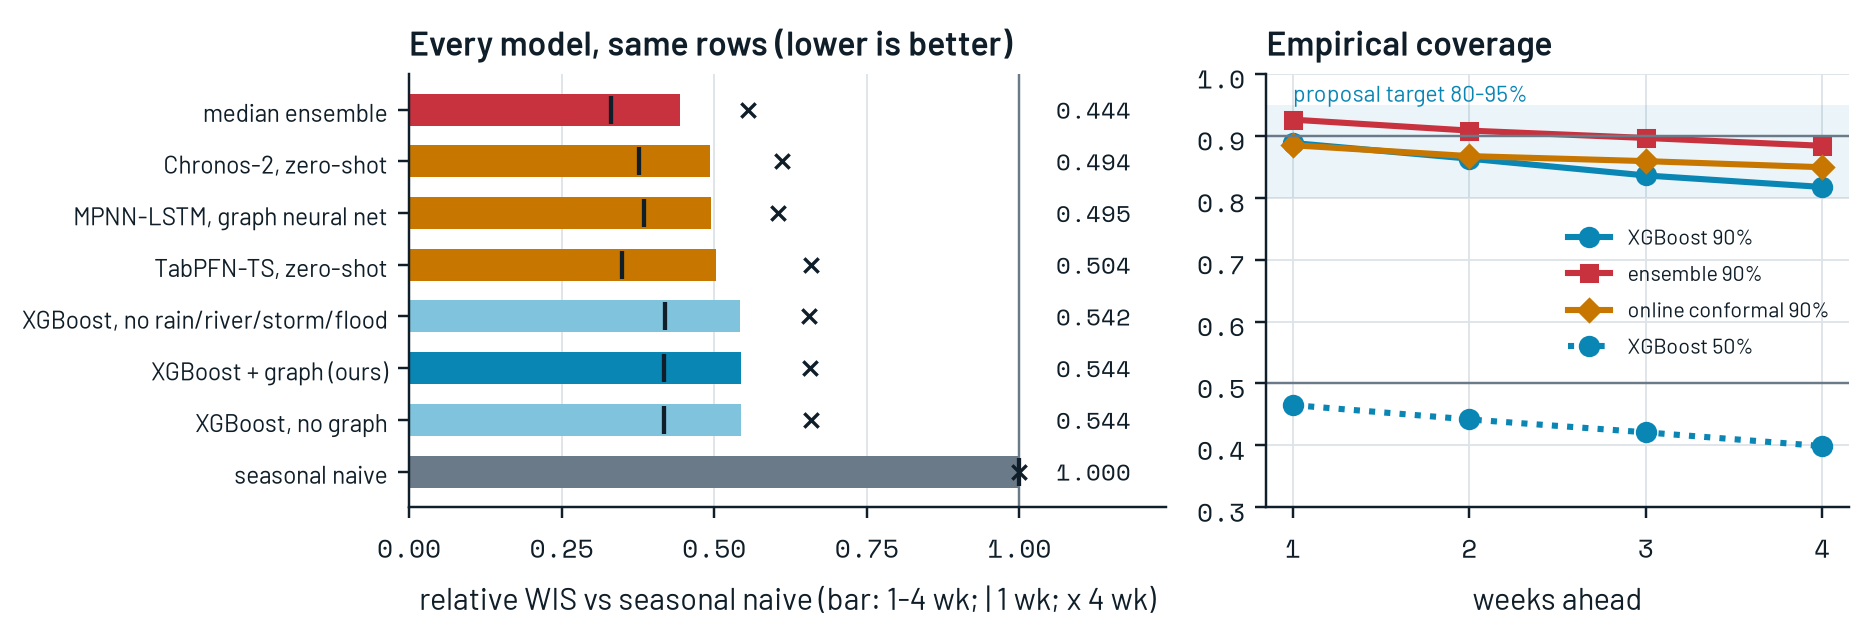
\includegraphics[width=\linewidth]{f03_wis}
\caption{Left: relative WIS of every model over one to four weeks (ticks: one and four weeks). Right: coverage against the nominal lines and the proposal's band.}
\label{fig:wis}
\end{figure}

\begin{itemize}
\item \textbf{Mean against median.} Every benchmark beats XGBoost on mean WIS, and the ensemble is best. On the median XGBoost is best (\mwXGB{} cases against \mwBenchRange{}; ensemble \mwEns{}). Split at the 90th percentile of weekly cases (\splitThr{}): below it the benchmarks' mean WIS is \splitLoRange{} times XGBoost's, above it \splitHiRange{} times. The better means come from the large-count epidemic weeks; the ensemble (\ensSplitLo{} below, \ensSplitHi{} above) gains in both.
\item \textbf{Chronos-2} as first specified, on $\log(1 + \text{incidence})$, collapsed on one-week reporting spikes (relative WIS \chronosLogRelWIS{}). The headline run uses the incidence scale with past-only covariates; it was chosen \emph{after} seeing that failure. Without covariates it scores \chronosNoCovRelWIS{}, so the covariates do not help.
\item \textbf{TabPFN-TS} runs univariate (it ignores past-only covariates) with the ungated TabPFN v2 regressor; the default v3.5 weights need a login and licence and were not used. A lagged-covariate variant scores \tabpfnLagCovRelWIS{}.
\item \textbf{MPNN-LSTM} uses border adjacency (\mpnnBorderEdges{} edges) plus ferry routes (\mpnnFerryEdges{} more, a 2024--2026 proxy); with no graph it scores \mpnnNoneRelWIS{}, the same within seed noise, in line with the sparse lead-lag graph.
\item \textbf{Where it is used.} The benchmarks and the ensemble exist only at the rolling-origin weeks of 2018--2019. Storm scenarios, shifted tracks, 2020 and the storm catalogue use XGBoost with calibrated $R$, because the zero-shot models take no storm-track input.
\end{itemize}

% !TEX root = ../main.tex
\section{Surge probability: calibration}
\label{sec:calibration}

The model's raw $R$ is \textbf{\ifRawUnderConfident under-confident\else over-confident\fi{} in the middle}: in the reliability bins between \gapBinLo{} and \gapBinHi{}, outcomes came true \ifRawUnderConfident more\else less\fi{} often than forecast, by up to \gapRaw{} (Figure~\ref{fig:reliability}). Isotonic regression maps raw $R$ to the observed surge frequency. It is fitted at each origin on earlier forecasts whose four-week outcome was already known (target week no later than the origin), so it never sees the future. It needs \calMinRows{} past outcomes first: the \nUncalOrigins{} origins before \firstCalOrigin{} keep raw $R$ (\nUncalRows{} rows). After recalibration the largest middle-bin gap is \gapCal{}\ifCalGapSmaller, smaller than before\else, no smaller than before\fi.

\begin{figure}[htbp]
\centering
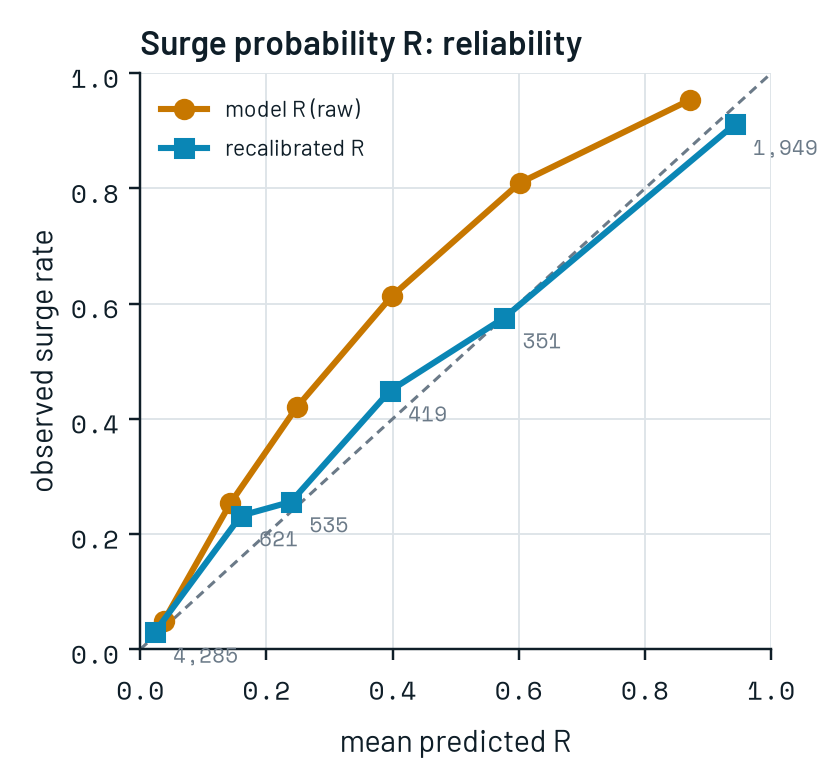
\includegraphics[width=0.5\linewidth]{f04_reliability}
\caption{Reliability of $R$ over the 2018--2019 unit-weeks, before (amber) and after (teal) isotonic recalibration; labels give the unit-weeks per bin.}
\label{fig:reliability}
\end{figure}

Table~\ref{tab:calib} gives the Brier scores: recalibration \ifCalImproves lowers\else raises\fi{} it from \brierRaw{} to \brierCal{} over all 2018--2019 origins. The base rate is \baseRatePct{}\ifBaseRateHigh, not \surgeExpected{}, because 2019 was an epidemic year and the thresholds come from earlier, quieter years\fi. The scenario files keep both \code{R} (calibrated, used for $P$ and the tiers) and \code{R\_raw}. Recalibration changes which provinces reach the provisional tiers (pre-position at $R \geq \tierPreR$, deploy at $R \geq \tierDeployR$ with $A \geq \tierDeployA$): for Ompong the mean $R$ \ifOmpongRRises rises\else falls\fi{} from \ompongRRaw{} to \ompongR{}. The tier thresholds still need review with users.

\begin{table}[htbp]
\centering
\caption{Brier score of $R$ before and after recalibration, against always predicting the base rate.}
\label{tab:calib}
\footnotesize
\begin{tabular}{@{}l r r r r r r r@{}}
\toprule
rows & $n$ & base rate & mean $R$ raw & mean $R$ cal. & Brier raw & Brier cal. & Brier base rate \\
\midrule
\tablerows{calib}
\bottomrule
\end{tabular}
\end{table}

\textbf{Ties.} Isotonic regression is a step function, so provinces share values: for Ompong the \nUnits{} units take \nDistinctR{} distinct values of $R$ and \nTies{} share the top value (\tieValue{}). A ranking by $R$ alone has ties; $P = R \times A$ breaks them by access, and the backtest's Spearman correlations use average ranks.

% !TEX root = ../main.tex
\section{The lead-lag graph}
\label{sec:leadlag}

In the final window (\llN{} series, $T = \llT$ weeks after seasonal differencing; Davao Occidental sits out with more than a tenth of its weeks missing), PCMCI+ keeps \textbf{\llEdges{}} lagged links between provinces at $q < \fdrQ$ (Figure~\ref{fig:leadlag} and Table~\ref{tab:edges}). Plain lagged cross-correlation with the same FDR filter keeps \textbf{\xcEdges{}}, because the 2019 national epidemic makes almost every pair of provinces move together.

The proposal's sentinel idea is therefore \textbf{weakly supported at province-week level}. The links are statistical dependencies, not evidence of transmission, and several join distant provinces. Likely reasons: weekly province totals average out local waves, four years is short for \llN{} series, and reporting artefacts dominate small provinces. Synchrony studies have found travelling dengue waves at longer time scales \parencite{vanpanhuis2015}. The MPNN-LSTM benchmark points the same way: its result does not depend on its graph.

\begin{figure}[htbp]
\centering
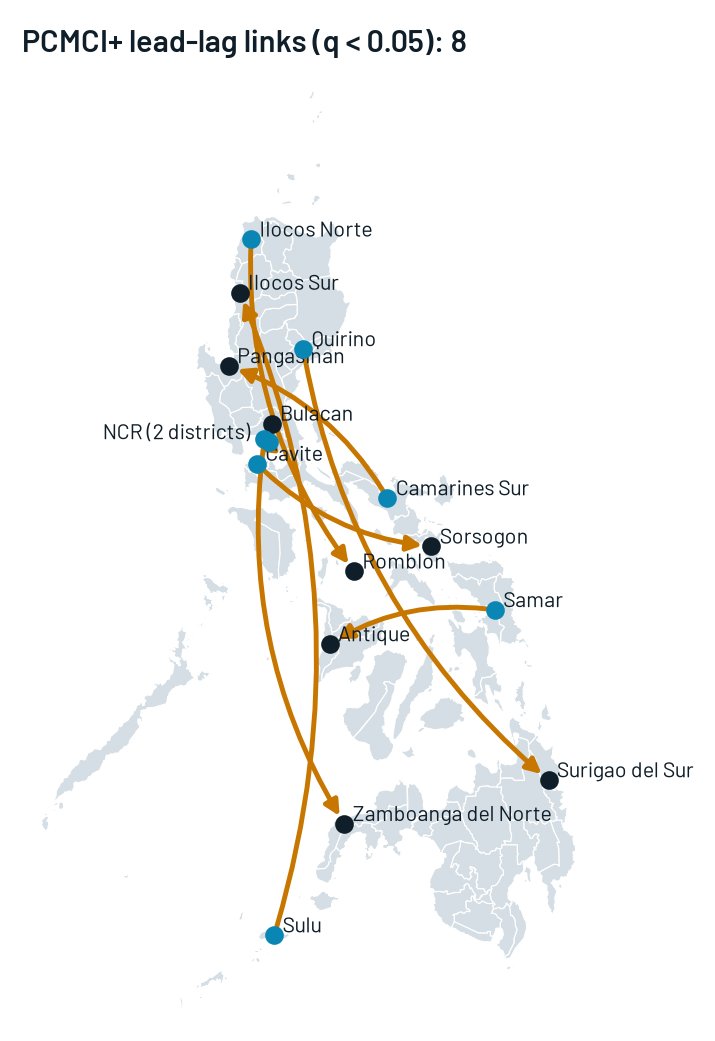
\includegraphics[width=0.48\linewidth]{f06_leadlag}
\caption{The PCMCI+ links learned on 2016--2019; teal nodes lead.}
\label{fig:leadlag}
\end{figure}

\begin{table}[htbp]
\centering
\caption{The lagged links PCMCI+ keeps, by strength: lag, partial correlation, FDR q-value and how often the link reappears over bootstrap resamples.}
\label{tab:edges}
\footnotesize
\begin{tabular}{@{}l l r r r r@{}}
\toprule
leader & follower & lag (wk) & partial corr. & $q$ & bootstrap freq. \\
\midrule
\tablerows{edges}
\bottomrule
\end{tabular}
\end{table}

% !TEX root = ../main.tex
\section{Observed flood: Sentinel-1}
\label{sec:flood}

Radar sees through typhoon clouds. For each typhoon, new open water is mapped on Google Earth Engine from the vertical-horizontal (VH) backscatter of Sentinel-1 in 100~m tiles near the track: the before image is the median of days $-30$ to $-3$ and the after image the darkest of days 0 to $+$\sOneAfterDays{}, \textbf{both from the same relative orbit}. A pixel is new flood when its VH backscatter drops by at least 3~dB and ends at most $-18$~dB; permanent water, slopes over 5\textdegree{} and specks under 8 pixels are removed \parencite[after][]{unspider}. The first version, an after-to-before ratio on decibel values with mixed orbits, recovered almost none of the EMS flood and was replaced.

Figure~\ref{fig:s1} maps the new-flood share per unit and Table~\ref{tab:s1} gives the people in new flood per storm. Table~\ref{tab:s1muni} repeats this per municipality; there $\rho$ is the Spearman correlation, over the municipalities the radar saw, between network access loss $A$ and the new-flood share. Access loss follows flood but not one-to-one: a municipality can be flooded and keep a dry road to a hospital.

\begin{figure}[htbp]
\centering
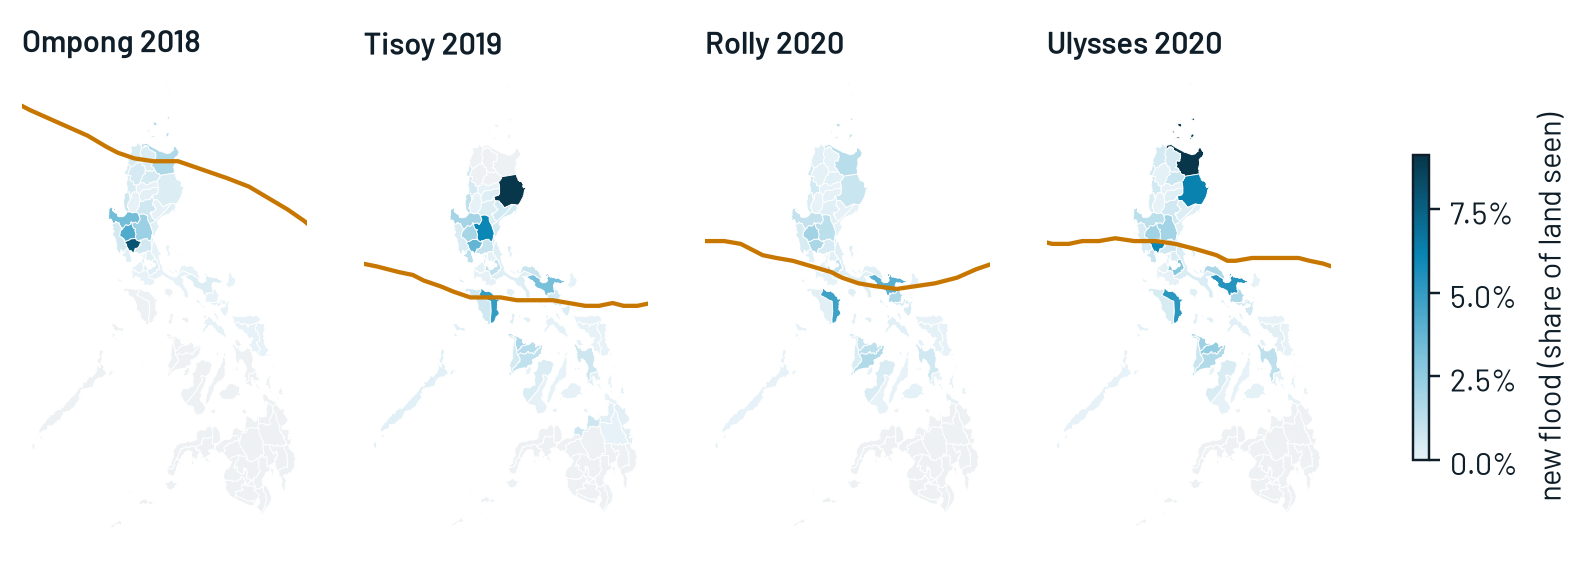
\includegraphics[width=\linewidth]{f11_s1_flood}
\caption{New-flood share of the land Sentinel-1 saw, per unit, with each typhoon's track.}
\label{fig:s1}
\end{figure}

\begin{table}[htbp]
\centering
\caption{People in new flood per typhoon, from the Sentinel-1 masks.}
\label{tab:s1}
\small
\begin{tabular}{@{}l r r r l@{}}
\toprule
typhoon & people in new flood & units $>$\sOneFloodThr{} flooded & max unit share & most people flooded \\
\midrule
\tablerows{s1}
\bottomrule
\end{tabular}
\end{table}

\begin{table}[htbp]
\centering
\caption{Sentinel-1 per municipality: municipalities seen over more than a fifth of their area, municipalities with more than \sOneFloodThr{} new flood, the three with most people in new flood, and the rank correlation of access loss with flood.}
\label{tab:s1muni}
\footnotesize
\begin{tabularx}{\linewidth}{@{}l r r L r@{}}
\toprule
typhoon & seen & flooded & most people in new flood: municipality (province), people, share & $\rho(A, \text{flood})$ \\
\midrule
\tablerows{s1muni}
\bottomrule
\end{tabularx}
\end{table}

\subsection{Checked against Copernicus EMS}

Inside the EMS areas of interest for Ompong, EMS mapped \emsKm{}~km\textsuperscript{2} of observed flood and Sentinel-1 flagged \sOneKm{}~km\textsuperscript{2}; \bothKm{}~km\textsuperscript{2} overlap. \textbf{\emsPrecision{}} of the Sentinel-1 flood there is confirmed by EMS, and Sentinel-1 recovers \textbf{\emsRecall{}} of the EMS area (Figure~\ref{fig:s1ems}).\ifEMSRecallLow{} Low recall is expected: EMS used other imagery and dates, while one Sentinel-1 orbit passed here only twice in the window.\fi

\begin{figure}[htbp]
\centering
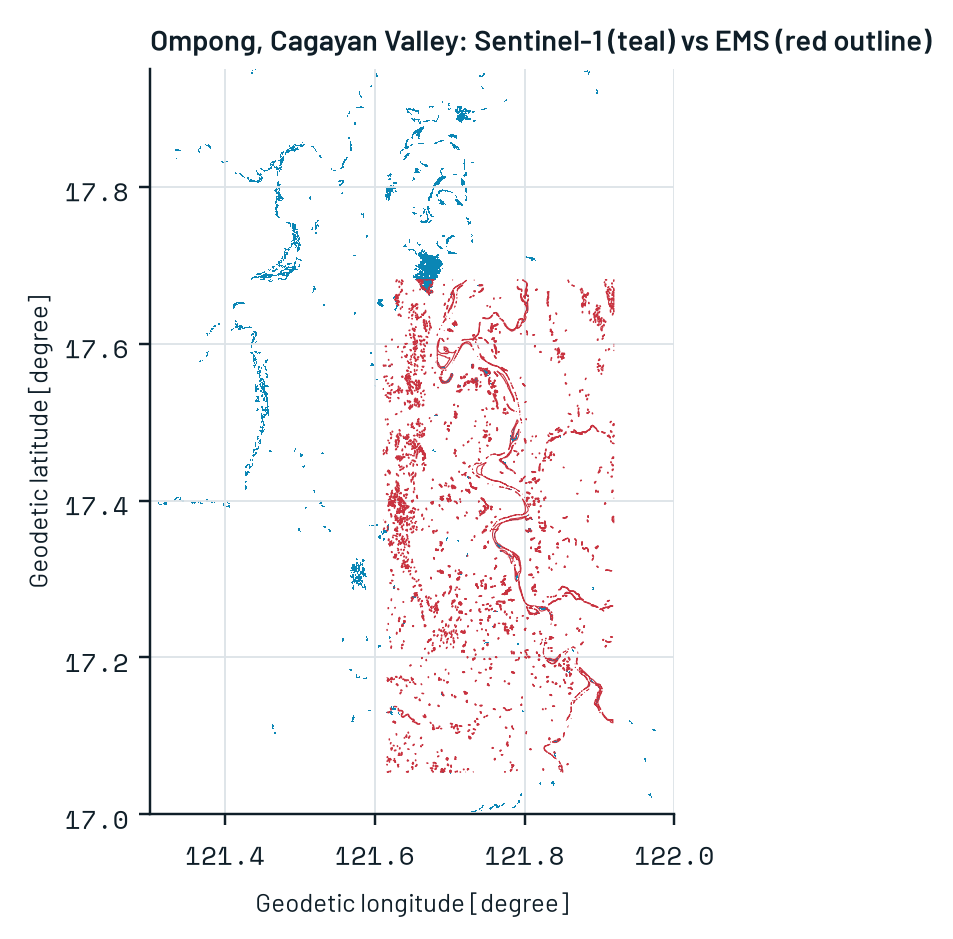
\includegraphics[width=0.55\linewidth]{f12_s1_ems}
\caption{Ompong around Tuguegarao: Sentinel-1 new flood (teal) and Copernicus EMS observed flood (red outlines).}
\label{fig:s1ems}
\end{figure}

% !TEX root = ../main.tex
\section{Access loss under four typhoons}
\label{sec:access}

\textbf{Baseline.} \cellsPopM{} people live in the 1~km cells. On the network, \routeShare{} of them have a road or ferry route to one of \nHosp{} hospitals, with a population-weighted mean trip of \meanHours{}~h; the raster reaches \rasterReach{} with a mean of \rasterHours{}~h. Results are also written for \nAdmThree{} municipalities. Figure~\ref{fig:network} shows the ferry routes and hospitals.

\begin{figure}[htbp]
\centering
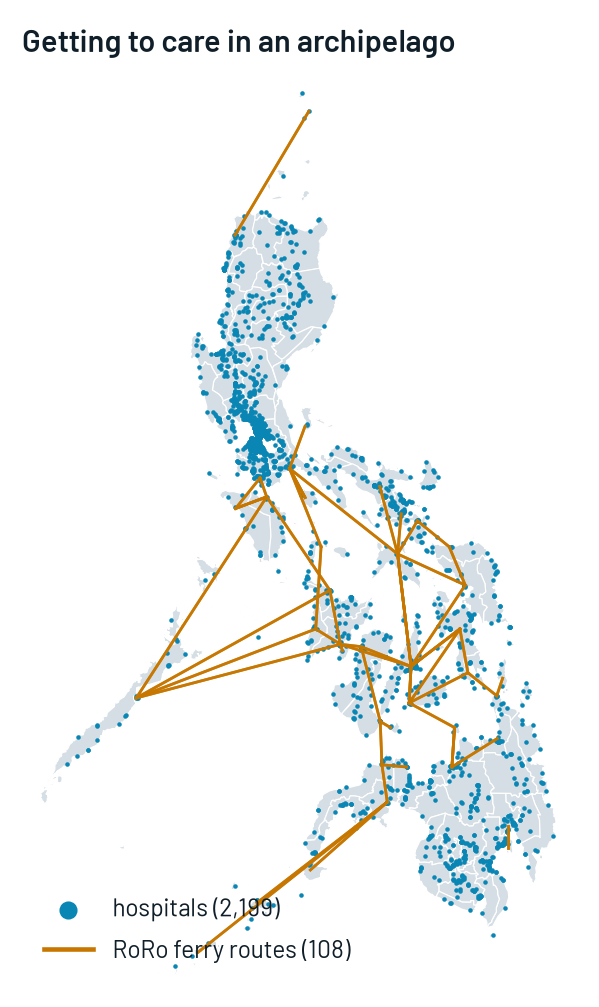
\includegraphics[width=0.45\linewidth]{f13_network}
\caption{Getting to care in an archipelago: the ferry routes (2024--2026 operations, a proxy for 2018--2020) and the fallback hospital list.}
\label{fig:network}
\end{figure}

Table~\ref{tab:methods} gives the people cut off by each method for the observed tracks, and Figure~\ref{fig:access} maps the network's access loss $A$ per unit.

\begin{table}[htbp]
\centering
\caption{People cut off per observed track: network, raster and the range of the per-unit minimum and maximum of the two; rank agreement of $A$ over units ($\rho$) and of $P$ (Kendall's $\tau$); top-ten provinces by $P$ shared; vulnerable people cut off (network).}
\label{tab:methods}
\footnotesize
\begin{tabular}{@{}l r r r r r r r r@{}}
\toprule
typhoon & network & raster & range & $\rho$ of $A$ & $\tau$ of $P$ & top-10 shared & under-5 & 60+ \\
\midrule
\tablerows{methods}
\bottomrule
\end{tabular}
\end{table}

\begin{figure}[htbp]
\centering
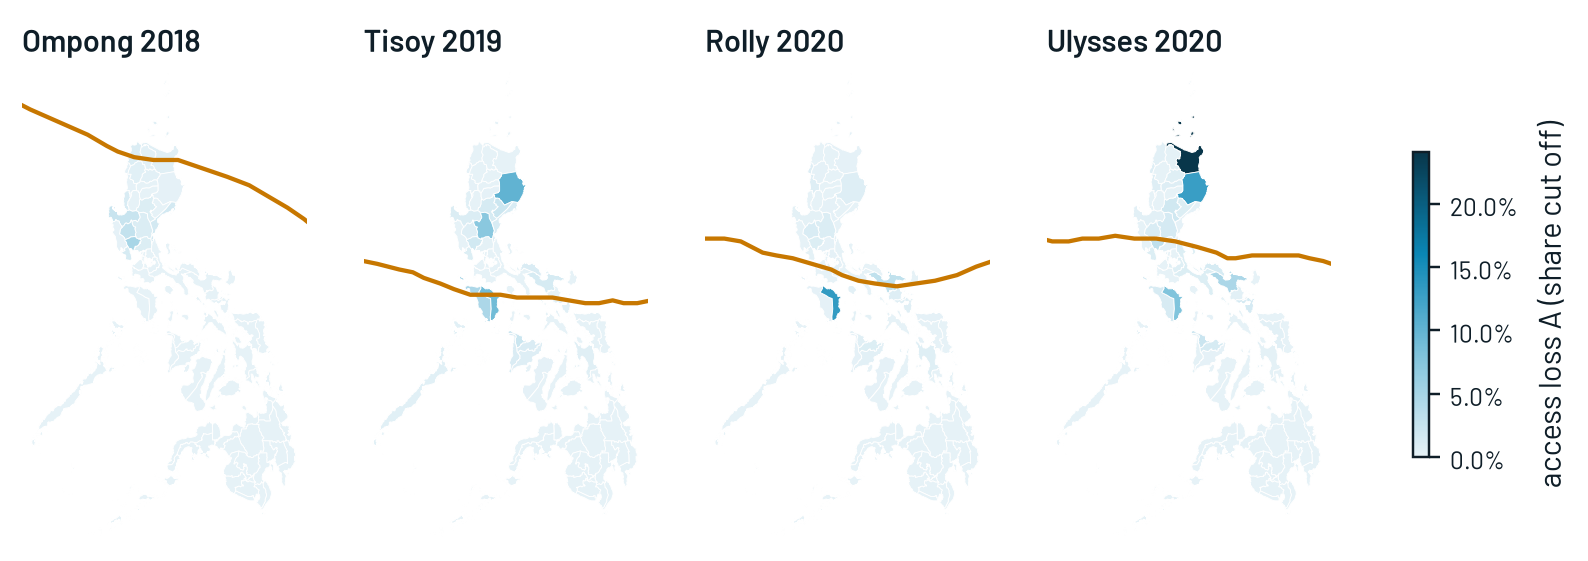
\includegraphics[width=\linewidth]{f08_access}
\caption{Network access loss $A$ per unit for the observed tracks. Roads are cut by Sentinel-1 observed flood; ferries crossing the gale swath are cancelled.}
\label{fig:access}
\end{figure}

\begin{note}
Observed tracks: roads are cut only where Sentinel-1 saw new water. Radar misses floods under dense vegetation, in built-up areas and between passes, so these are \textbf{lower bounds}. The \nProxy{} shifted tracks have no image and use the NOAH 25-year proxy (every high-hazard road in the swath cut): \proxyCutRange{} people cut off on the network, an \textbf{upper bound}. Ferry routes are 2024--2026 operations, a proxy for 2018--2020. $A$ uses radar that exists up to \sOneAfterDays{} days after the forecast origin: it is a retrospective access estimate.
\end{note}

\subsection{Network against friction raster}

The proposal runs a raster method next to the network because OSM completeness is uneven, and reports their disagreement as uncertainty. Both use the same hospitals, population cells, ferry lines and storm rules.

\textbf{On a normal day} the raster reaches \ifRasterReachMore more\else fewer\fi{} people (\rasterReach{} against \networkReach{}) and is \ifRasterFaster faster\else slower\fi{} (population-weighted mean \rasterHours{}~h against \networkHours{}~h; median cell ratio of raster to network \medianRatioBase{})\ifRasterFaster: it can cross land without a mapped road\fi. The two rank places \ifMethodsRankAlike alike\else differently\fi: Spearman \spearmanCells{} over the \cellsBoth{} cells that both reach, and \spearmanUnits{} over the \nUnits{} units' mean trip.

\textbf{Under a storm} (Figure~\ref{fig:methods}), with Sentinel-1 flood the raster cuts off \ifRasterMoreSOne more\else fewer\fi{} people than the network (\cutRasterRange{} against \cutNetRange{}); with the NOAH proxy it cuts off \ifRasterMoreProxy more\else fewer\fi{} (median ratio \proxyRatio{}).\ifRasterMoreSOne\ifRasterMoreProxy\else{} The gap changes sign with the flood source. A likely reason: at 1~km a flooded cell centre closes the whole cell, while radar flood is patchy and the network closes only the flooded road edges; the proxy closes every high-hazard road, which the raster's cell-centre test samples more sparsely.\fi\fi{} The unit rankings of $A$ have $\rho$ \rhoProxyRange{} under the proxy and \rhoObsRange{} with radar\ifProxyAgreesBetter{} (they agree better under the proxy)\fi, and with radar \topTenSharedRange{} of the top-ten provinces by $P$ are shared. The dashboard shows $A$ and $P$ with this range. On the raster method the sensitivity analysis of Section~\ref{sec:validation} gives Kendall's $\tau \geq \tauMinRaster$.

\begin{figure}[htbp]
\centering
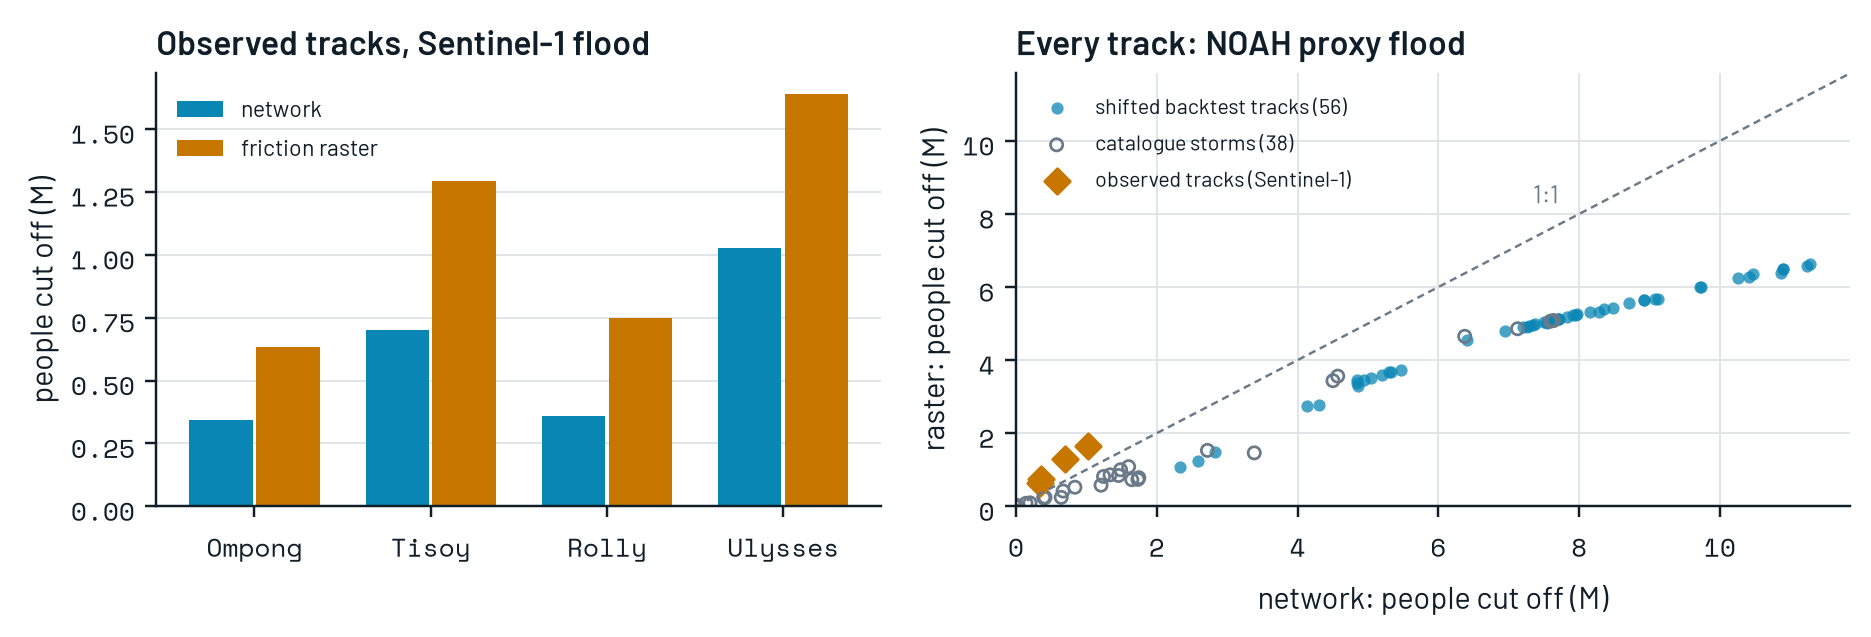
\includegraphics[width=\linewidth]{f15_methods}
\caption{People cut off by each method. Left: observed tracks with Sentinel-1 flood. Right: every track that uses the NOAH proxy (shifted backtest tracks and catalogue storms), with the 1:1 line.}
\label{fig:methods}
\end{figure}

\subsection{Vulnerable groups}

HRSL puts \uFiveShare{} of people under five and \oSixtyShare{} aged 60 or over; the 2020 census has \censusUFive{} and \censusSixty{}. \ifHRSLUnderOld HRSL therefore \textbf{under-counts older people}\ifHRSLOverYoung{} (and over-counts young children)\fi, so the 60+ cut-off numbers are low estimates.\fi{} Among those cut off, the under-5 share is \uFiveCutRange{} and the 60+ share \oSixtyCutRange{}.

% !TEX root = ../main.tex
\section{Priority scenarios}
\label{sec:priority}

Table~\ref{tab:storms} summarises the four backtest typhoons on their observed tracks: ferry routes cancelled, people cut off on the network, mean $A$ and $R$ over the \nUnits{} units, the number of provinces in the two action tiers, and the province ranked first.

\begin{table}[htbp]
\centering
\caption{The four backtest typhoons, observed tracks (local name, with the international name and season).}
\label{tab:storms}
\footnotesize
\begin{tabularx}{\linewidth}{@{}L r r r r c L@{}}
\toprule
typhoon & ferry routes cut & people cut off & mean $A$ & mean $R$ & deploy / pre-position & top priority \\
\midrule
\tablerows{storms}
\bottomrule
\end{tabularx}
\end{table}

\subsection{Ompong 2018}

Ompong made landfall in Cagayan on \landfallOmpong{}. The model, trained on data to the landfall week only, puts \textbf{\topOmpong{}} first, with \deployOmpong{} provinces in the \enquote{deploy mobile clinics} tier and \preposOmpong{} in \enquote{pre-position supplies} (Figure~\ref{fig:priority}). \enquote{Deploy} needs at least \tierDeployA{} of people cut off. Of the four observed tracks, with observed flood, \nStormsDeploy{} put any province there; the hazard-proxy shifted tracks of Ompong put \proxyDeployOmpong{} provinces there. Figure~\ref{fig:scatter} places every unit on the risk and access axes with the provisional tier thresholds.

The dashboard repeats this for every storm and \nShifted{} shifted variants of each track ($\pm$\shiftLat\textdegree{} north or south, $\pm$\shiftLon\textdegree{} east or west), so a health officer can ask \enquote{what if it comes in further south?} and get an answer in seconds.

\begin{figure}[htbp]
\centering
\begin{minipage}[t]{0.47\linewidth}
\centering
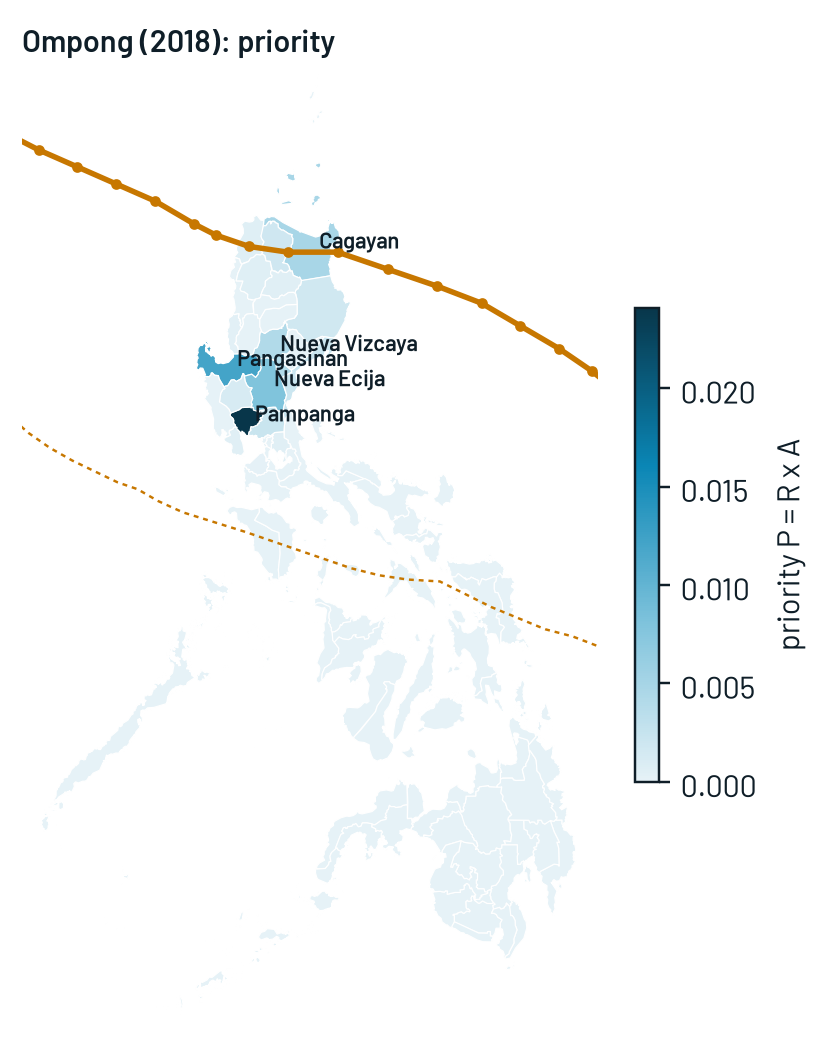
\includegraphics[width=\linewidth]{f07_priority_ompong}
\caption{$P = R \times A$ for Ompong with its track and gale swath; the top five are labelled.}
\label{fig:priority}
\end{minipage}\hfill
\begin{minipage}[t]{0.5\linewidth}
\centering
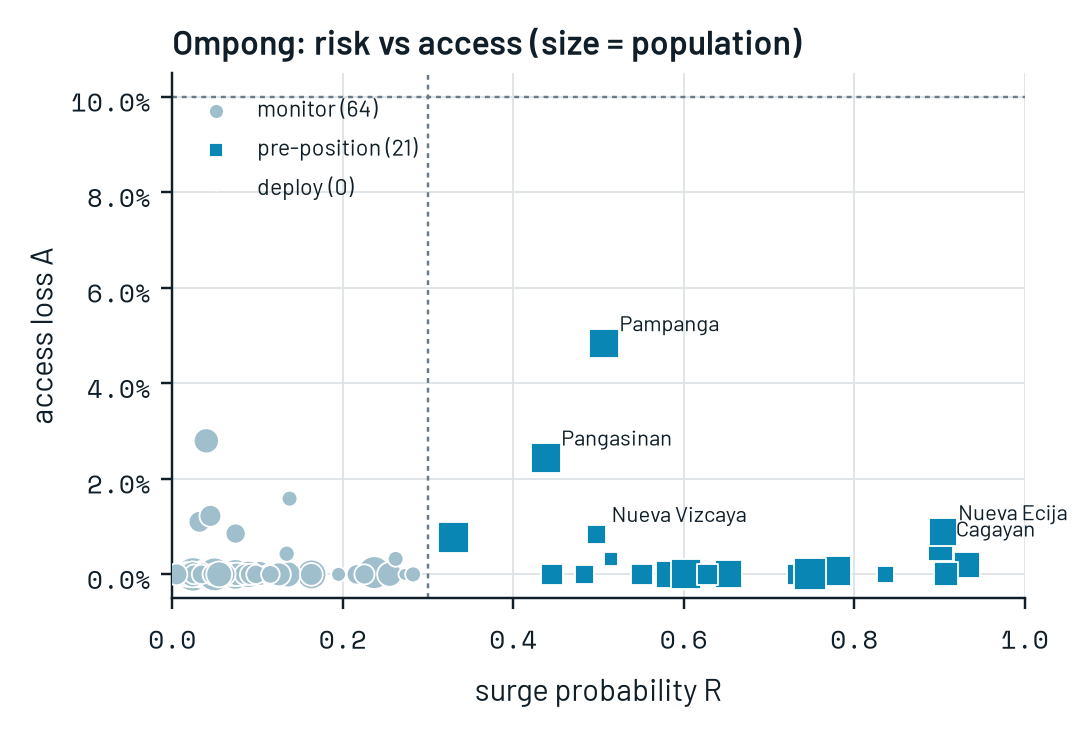
\includegraphics[width=\linewidth]{f09_scatter}
\caption{Risk against access for Ompong. Dotted lines are the provisional tier thresholds ($R = \tierPreR$, $A = \tierDeployA$); marker shape gives the tier.}
\label{fig:scatter}
\end{minipage}
\end{figure}

\subsection{Every storm, \catYearMin--\catYearMax}
\label{sec:catalog}

Beyond the four backtests, the build scores the observed track of every other storm whose gale swath touched Philippine land: \textbf{\nCat{} storms}. Each uses the latest model fitted before its week (never later data), $R$ calibrated where enough past outcomes exist (\nCalCat{} of \nCat{}), and \textbf{the NOAH 25-year proxy for flood}, since no radar map exists for them, so their cut-off counts are upper bounds. \nSkipped{} storms of 2016 are skipped: their model would have under \minHistory{} weeks of history. Figure~\ref{fig:catalog} plots risk against people cut off for all \nAllStorms{} storms and Table~\ref{tab:catalog} lists them.

\begin{figure}[htbp]
\centering
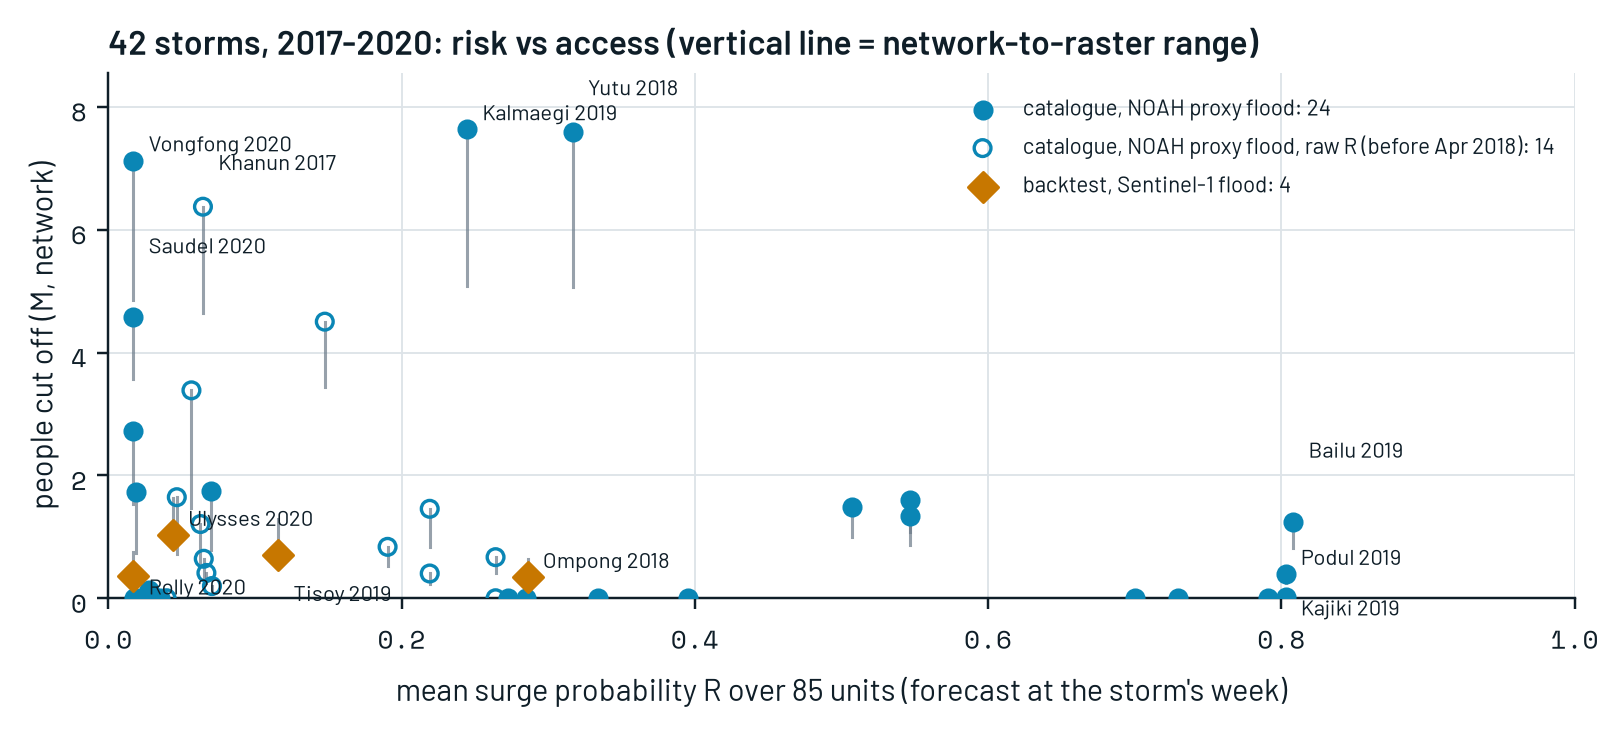
\includegraphics[width=\linewidth]{f16_catalog}
\caption{Mean surge probability and people cut off per storm. Diamonds: the four backtests (Sentinel-1 flood, lower bounds); circles: catalogue storms (NOAH proxy, upper bounds); hollow: raw $R$. The vertical line spans the network-to-raster range.}
\label{fig:catalog}
\end{figure}

\begin{table}[htbp]
\centering
\caption{Every scored storm in date order. $R$: mean over the \nUnits{} units; cut: people cut off (millions), network and raster; $R \times$cut: expected people at surge risk who are cut off ($\Sigma\, R \times$ cut off over units); D/P: provinces at deploy / pre-position. $\blacklozenge$ backtest (Sentinel-1); \textsuperscript{\dag} raw $R$ (before calibration was possible).}
\label{tab:catalog}
\scriptsize
\begin{tabular}[t]{@{}l r r r r r r@{}}
\toprule
storm & $R$ & cut & raster & $R \times$cut & ferry & D/P \\
\midrule
\tablerows{catalogA}
\bottomrule
\end{tabular}\hfill
\begin{tabular}[t]{@{}l r r r r r r@{}}
\toprule
storm & $R$ & cut & raster & $R \times$cut & ferry & D/P \\
\midrule
\tablerows{catalogB}
\bottomrule
\end{tabular}
\end{table}

The largest cut-offs (\largestCutStorms{}) pair with low $R$; the high-$R$ storms (\highRStorms{}) came in the 2019 epidemic season. The network and raster agree across units with a median $\rho$ of \catRhoMedian{} (minimum \catRhoMin{}) over the \catRhoN{} storms with any cut-off.

% !TEX root = ../main.tex
\section{Validation, sensitivity and benchmark}
\label{sec:validation}

\subsection{Did high-priority provinces see more cases?}

For each typhoon, the ranking made at the landfall week is compared with the incidence each unit saw over the next four weeks, relative to its own threshold (Table~\ref{tab:valid}, Figure~\ref{fig:valid}). $R$ ranks provinces well for both 2018--2019 storms. $P$ correlates less with cases, as it should: $A$ measures access, not disease. After Ompong, \topTenSurgedOmpong{} of the ten highest-priority provinces surged against a \surgeRateOmpong{} base rate. After Tisoy almost nothing surged (the 2019 season was over), so the top-ten rate is zero and the Brier score is low for the right reason.

\begin{table}[htbp]
\centering
\caption{Backtest per typhoon: units scored, share that surged, Spearman correlation of $R$ and of $P$ with the observed incidence, surge rate among the ten highest-priority units, and the Brier score of $R$.}
\label{tab:valid}
\footnotesize
\begin{tabularx}{\linewidth}{@{}l l r r r r r r L@{}}
\toprule
typhoon & origin & units & surged & $\rho(R, \text{obs})$ & $\rho(P, \text{obs})$ & top-10 surged & Brier $R$ & note \\
\midrule
\tablerows{valid}
\bottomrule
\end{tabularx}
\end{table}

\begin{figure}[htbp]
\centering
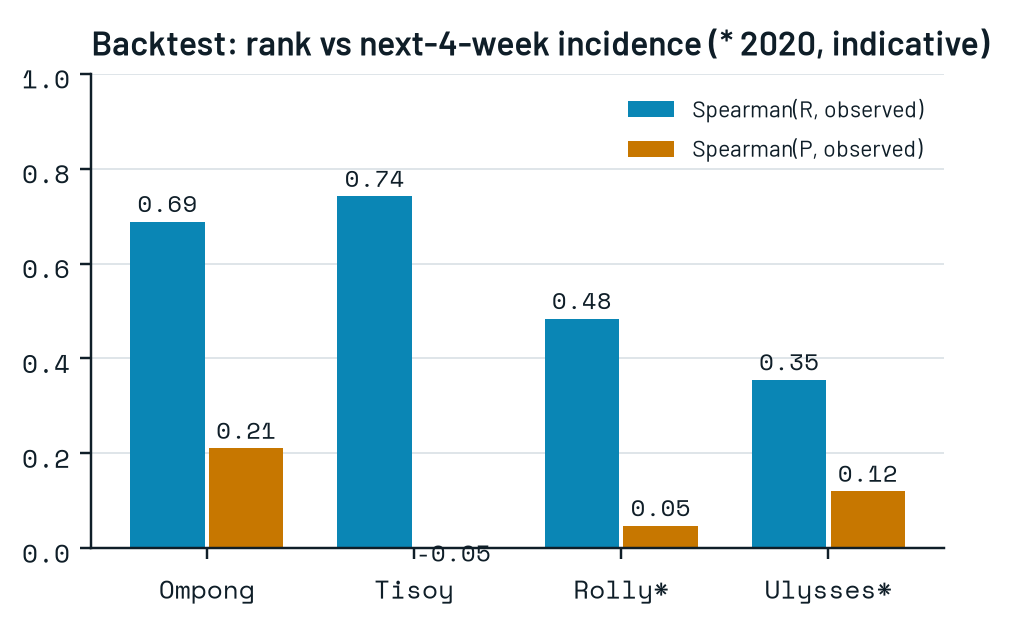
\includegraphics[width=0.62\linewidth]{f10_validation}
\caption{Spearman correlation of each ranking (calibrated $R$) with the observed incidence over the next four weeks, relative to each unit's threshold. Starred storms (2020) are indicative only.}
\label{fig:valid}
\end{figure}

\subsection{Sensitivity}

Table~\ref{tab:sens} gives Kendall's $\tau$ between the base ranking by $P$ (network method) and the ranking under each changed setting. Every variant changes $A$ a little but none reorders the ranking: the spread of $P$ is dominated by $R$. The same variants on the raster method give $\tau \geq \tauMinRaster$. The gale fallback never triggers for these storms.

\begin{table}[htbp]
\centering
\caption{Sensitivity: Kendall's $\tau$ of $P$ against the base settings (network method), and Ompong's mean $A$ under each variant.}
\label{tab:sens}
\footnotesize
\begin{tabular}{@{}l r r r r r@{}}
\toprule
variant & Ompong $\tau$ & Tisoy $\tau$ & Rolly $\tau$ & Ulysses $\tau$ & mean $A$ (Ompong) \\
\midrule
\tablerows{sens}
\bottomrule
\end{tabular}
\end{table}

\subsection{Metro Manila benchmark}

Cutting every road of the National Capital Region (NCR) in NOAH 25-year medium or high hazard leaves \textbf{\benchNCR{}} of NCR without a route within the cut-off rule. A study of the same region reported \litNCRShare{} of people losing access to higher-level care at a 15~cm flood \parencite{tariverdi2023}. The flood and facility definitions differ, so this is an order-of-magnitude check only.

% !TEX root = ../main.tex
\section{Leptospirosis: the stretch goal}
\label{sec:lepto}

The proposal assumed that no open subnational leptospirosis series exists. Project CCHAIN on HDX has weekly counts from the Philippine Integrated Disease Surveillance and Response (PIDSR) system for \leptoNCities{} cities, and a national weekly series of notifiable diseases is published on Mendeley Data. Both are analysed as \textbf{retrospective associations}, not forecasts: negative-binomial models of weekly cases on CHIRPS rain 0 to \leptoMaxLag{} weeks earlier, with seasonal terms, year and city effects and a COVID-19 term. Figure~\ref{fig:lepto} shows the incidence rate ratios (IRR) by lag.

\begin{figure}[htbp]
\centering
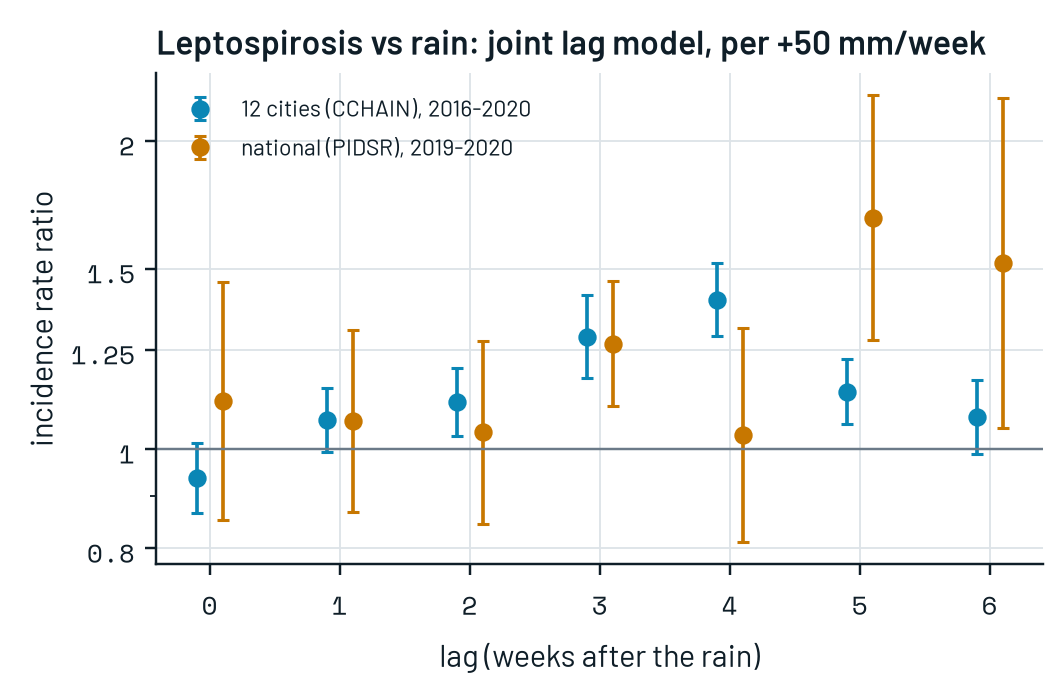
\includegraphics[width=0.72\linewidth]{f17_lepto}
\caption{Joint distributed-lag incidence rate ratios (95\% confidence intervals) per +\leptoRainPer{}~mm/week of rain, for the cities and the national series.}
\label{fig:lepto}
\end{figure}

\begin{itemize}
\item \textbf{Cities (\cityObs{} city-weeks, \cityCases{} cases, 2016--2020): the headline.} Rain is followed by leptospirosis \citySigRange{} weeks later; the joint peak is at lag \cityPeakLag{}, IRR \cityPeakCI{} per +\leptoRainPer{}~mm/week, and the cumulative IRR over lags 0 to \leptoMaxLag{} is \cityCumCI{}. A heavy-rain week (at or above the city's \leptoHeavyPctl{} percentile) peaks at lag \heavyPeakLag{}: \heavyPeakCI{}. That is a week or two later than the peak of \litLeptoPeak{} found in an earlier Philippine study \parencite{matsushita2018}; the CCHAIN week label is uncertain by about a week.
\item \textbf{National (\natObs{} weeks, 2019--2020): consistent, weaker.} The joint peak is at lag \natPeakLag{}, \natPeakCI{}; the cumulative IRR is \natCumCI{}. With 2019 alone the cumulative effect is \natNineteenCumCI{}: much of the national signal comes from 2020 (the December surge after Rolly and Ulysses, under COVID-19 reporting).
\item \textbf{Typhoons: mixed.} After Rolly and Ulysses (2020), cities inside the gale swath had \didRUPost{} times the outside cities' ratio of observed to expected cases in weeks 1 to 4 (pre-landfall placebo \didRUPre{}). For Ompong and Tisoy the ratio is \didOTPost{} but the placebo fails (\didOTPre{}): weeks of monsoon rain had already raised cases before Ompong. Four storms and \leptoNCities{} cities support no general storm effect.
\item \textbf{Flood: not estimable.} Of \sOnePairs{} city-storm pairs, \sOnePairsSeen{} had radar over more than a fifth of the city and \sOnePairsFlooded{} show any new flood (at most \sOnePairsMax{}): too few to relate flood to cases. Flood mediation stays an assumption from the literature.
\end{itemize}

The \leptoNCities{} cities are not a sample of provinces, so nothing here is extrapolated to provinces, and leptospirosis is not in the dashboard's ranking.

% !TEX root = ../main.tex
\section{Scorecard against the proposal}
\label{sec:scorecard}

Table~\ref{tab:scorecard} sets each objective of the proposal against the result of this build. The status words are decided from the outputs present when the specification is generated.

\begin{table}[htbp]
\centering
\caption{Proposal objectives and the result in this build.}
\label{tab:scorecard}
\footnotesize
\begin{tabularx}{\linewidth}{@{}>{\raggedright\arraybackslash}p{0.27\linewidth} L l >{\raggedright\arraybackslash}p{0.24\linewidth}@{}}
\toprule
objective (proposal) & result in this build & status & note \\
\midrule
Province-week panel 2016--2020 on PSGC: dengue, rain, Sentinel-1, hazard, storms & \nUnits{} harmonised units $\times$ \nWeeks{} weeks; every listed layer plus river routing & \statusPanel & \nUnits{} harmonised 2016--2020 units, not \proposalProvinces{} provinces (\dgUnits{} reporting units); Sentinel-1 only in the four storm windows \\
Lead-lag graph (PCMCI+), sentinels (PageRank), communities (Louvain); test sentinel features out of sample & \llEdges{} links at $q < \fdrQ$; sentinels and communities on the dashboard; ablation run & \stOk & tested and null: graph against no graph, relative WIS \relWISGraph{} \\
Relative WIS below 1 against seasonal naive, 2018--2019 & XGBoost \relWIS{}; median ensemble \ensRelWIS{} & \stOk & \\
90\% interval coverage of \targetCov{} & \covNinety{} overall; \covNinetyRange{} by horizon & \stOk & four-week horizon close to the floor \\
Benchmarks: Chronos-2, TabPFN-TS, MPNN-LSTM; median ensemble; conformal check & all three and the ensemble scored on the same rows; online conformal check & \statusBench & the ensemble is evaluated, but storm scenarios use XGBoost (the zero-shot models take no storm-track input) \\
Access loss per municipality, friction-surface and network methods, four typhoons & both methods, \nAdmThree{} municipalities, four storms $\times$ \nTracks{} tracks & \statusAccess & method disagreement reported as the $A_{\text{lo}}$--$A_{\text{hi}}$ range \\
Sensitivity bounds (Kendall's $\tau$); Metro Manila benchmark & two methods, $\tau \geq \tauMinAll$; NCR \benchNCR{} against \litNCRShare{} & \stOk & order-of-magnitude check \\
Dashboard: ranked provinces, calibrated risk, access, sentinels, drivers, tier, any historical or shifted track & \nScen{} backtest scenarios and \nCat{} catalogue storms, pre-computed; $R$ recalibrated & \stOk & tiers are provisional rules \\
Backtest: did high-priority provinces see more cases? & $\rho(R)$ \rhoRRange{} over four storms & \stOk & 2020 storms indicative only (COVID-19 reporting) \\
System Usability Scale from three target users & test form and task built into the dashboard; \susN{} responses so far & \statusSUS & needs sessions with health and disaster-office users \\
Leptospirosis (stretch): national lag analysis; region-week series if digitised & national lag analysis, an open \leptoNCities{}-city series and a typhoon event study & \statusLepto & association only, not in the forecast; no province-level series \\
\bottomrule
\end{tabularx}
\end{table}

\subsection{Proposal corrections found in the data}

\begin{itemize}
\item \dgUnits{} dengue reporting units, not \proposalProvinces{} provinces (harmonised to \nUnits{}); deaths are unreliable; 2020 collapsed under COVID-19.
\item An open subnational leptospirosis series exists (Project CCHAIN, \leptoNCities{} cities).
\item The EMS activation for Rolly has damage grading only, no flood delineation; the Global Flood Database has no Philippine event after 2017 \parencite{tellman2021}.
\item The flood hazard maps come from the NOAH archive at 5 and 25 years, not the national lidar portal; \nHazNoMap{} units have no 25-year map.
\item HydroRIVERS places the Philippines in the Australasia file, not the Asia file.
\item The ferry routes describe 2024--2026 operations with partly coarse port coordinates; the official facility registry blocks scripted download (the OSM and NOAH fallback is used).
\item HRSL under-counts people aged 60 or over against the 2020 census.
\item The proposal's final forecast was the median ensemble; storm scenarios use XGBoost, the only storm-conditioned model.
\end{itemize}

% !TEX root = ../main.tex
\section{Limitations and next steps}
\label{sec:limits}

\subsection{Threats to validity}

\begin{itemize}
\item \textbf{Two evaluation years.} 2018--2019 contains one epidemic; the model ranking changes between mean and median WIS because of it.
\item \textbf{Surveillance artefacts.} Reporting delays and under-reporting are in the target; the forecasts predict reported, not true, cases.
\item \textbf{Observed flood.} Sentinel-1 sees each place every 6 to 12 days and misses flooding under dense vegetation and in built-up areas; the shifted tracks and the catalogue fall back to static hazard maps.
\item \textbf{Network gaps.} OSM completeness is uneven outside Luzon (the raster method bounds this); the ferries are 2024--2026 routes; the hospitals are an OSM and NOAH fallback without facility level or capacity. HRSL under-counts older people.
\item \textbf{Provisional rules.} The tier thresholds, road speeds and the cut-off rule are assumptions, partly addressed by the sensitivity analysis.
\item \textbf{Causality.} The PCMCI+ links and the leptospirosis lags are associations, not transmission routes or causal effects.
\end{itemize}

\subsection{Next steps}

\begin{enumerate}
\item Run the System Usability Scale test with three users from regional health offices, local government health units and disaster risk reduction offices \parencite{brooke1996}, and review the tiers with them.
\item Feed a forecast track from the national weather service and its cone of uncertainty in place of the historical shifts.
\item Add a second radar or optical source between Sentinel-1 passes.
\item Replace the hospital fallback with the official facility registry (facility level, so that access can mean a higher-level hospital).
\item Give the benchmarks storm inputs, or blend the ensemble with the storm signal of XGBoost, so that the scenarios can use the ensemble.
\end{enumerate}

\subsection{Reproducibility}

\code{setup.bat} (or \code{download\_data.bat}) $\rightarrow$ \code{build.bat} $\rightarrow$ \code{run\_app.bat}. The evaluation report and the slides are regenerated with \code{python scripts/make\_results.py}, and this specification with \code{python scripts/make\_spec.py}. Missing inputs are skipped, listed in \code{data/processed/status.json} and on the dashboard; re-running after they arrive needs no code change.


\printbibliography[heading=bibnumbered]

\appendix
% !TEX root = ../main.tex
% Sorted by the expanded name, not by the acronym. Add an entry whenever the text introduces a new acronym.
\section{Acronyms}
\label{sec:acronyms}

\begin{description}[style=nextline,leftmargin=2em,itemsep=0.2ex]
\item[Climate Hazards Group InfraRed Precipitation with Station data (CHIRPS)] Daily satellite-and-gauge rainfall on a grid of about 5~km; the main rain input.
\item[Common Operational Dataset of Administrative Boundaries (COD-AB)] The current boundary set; its codes are the join key.
\item[Copernicus Emergency Management Service (EMS)] Rapid flood mapping used to check Sentinel-1 for Ompong.
\item[Department of Health (DOH)] Publisher of the weekly dengue series that is the forecast target.
\item[False discovery rate (FDR)] The Benjamini--Hochberg control applied to the lead-lag links.
\item[High Resolution Settlement Layer (HRSL)] Population grids by age group, used for under-5 and 60+ people.
\item[Humanitarian Data Exchange (HDX)] The open data portal hosting the dengue, census, boundary and city series.
\item[Humanitarian OpenStreetMap Team (HOT)] Publisher of the OSM health facility extract used as hospitals.
\item[Incidence rate ratio (IRR)] The multiplicative change in cases per unit of exposure in the leptospirosis models.
\item[Integrated Multi-satellitE Retrievals for the Global Precipitation Measurement mission (IMERG)] Satellite rainfall, the second rain input.
\item[International Best Track Archive for Climate Stewardship (IBTrACS)] Storm tracks and gale radii.
\item[Japan Meteorological Agency (JMA)] Source of the 30-knot radius used when the United States radius is missing.
\item[Malaria Atlas Project (MAP)] Publisher of the friction surface behind the raster access method.
\item[Message-passing neural network with long short-term memory (MPNN-LSTM)] The graph neural network benchmark.
\item[National Capital Region (NCR)] Metro Manila, the access benchmark.
\item[Nationwide Operational Assessment of Hazards (NOAH)] Flood hazard maps per province; the flood proxy.
\item[OpenStreetMap (OSM)] The road network and part of the hospital list.
\item[Philippine Integrated Disease Surveillance and Response (PIDSR)] The surveillance system behind the city leptospirosis series.
\item[Philippine Standard Geographic Code (PSGC)] The national place code; COD-AB codes follow it.
\item[Roll-on/roll-off (RoRo)] Vehicle ferries; their routes are edges of the access network.
\item[Shapley additive explanations (SHAP)] Per-forecast feature attributions shown as drivers.
\item[Vertical-horizontal (VH)] The Sentinel-1 polarisation used for flood detection.
\item[Weighted interval score (WIS)] The proper score of a quantile forecast; lower is better.
\end{description}


\end{document}
